\documentclass{article}\usepackage[]{graphicx}\usepackage[]{color}
% maxwidth is the original width if it is less than linewidth
% otherwise use linewidth (to make sure the graphics do not exceed the margin)
\makeatletter
\def\maxwidth{ %
  \ifdim\Gin@nat@width>\linewidth
    \linewidth
  \else
    \Gin@nat@width
  \fi
}
\makeatother

\definecolor{fgcolor}{rgb}{0.345, 0.345, 0.345}
\newcommand{\hlnum}[1]{\textcolor[rgb]{0.686,0.059,0.569}{#1}}%
\newcommand{\hlstr}[1]{\textcolor[rgb]{0.192,0.494,0.8}{#1}}%
\newcommand{\hlcom}[1]{\textcolor[rgb]{0.678,0.584,0.686}{\textit{#1}}}%
\newcommand{\hlopt}[1]{\textcolor[rgb]{0,0,0}{#1}}%
\newcommand{\hlstd}[1]{\textcolor[rgb]{0.345,0.345,0.345}{#1}}%
\newcommand{\hlkwa}[1]{\textcolor[rgb]{0.161,0.373,0.58}{\textbf{#1}}}%
\newcommand{\hlkwb}[1]{\textcolor[rgb]{0.69,0.353,0.396}{#1}}%
\newcommand{\hlkwc}[1]{\textcolor[rgb]{0.333,0.667,0.333}{#1}}%
\newcommand{\hlkwd}[1]{\textcolor[rgb]{0.737,0.353,0.396}{\textbf{#1}}}%
\let\hlipl\hlkwb

\usepackage{framed}
\makeatletter
\newenvironment{kframe}{%
 \def\at@end@of@kframe{}%
 \ifinner\ifhmode%
  \def\at@end@of@kframe{\end{minipage}}%
  \begin{minipage}{\columnwidth}%
 \fi\fi%
 \def\FrameCommand##1{\hskip\@totalleftmargin \hskip-\fboxsep
 \colorbox{shadecolor}{##1}\hskip-\fboxsep
     % There is no \\@totalrightmargin, so:
     \hskip-\linewidth \hskip-\@totalleftmargin \hskip\columnwidth}%
 \MakeFramed {\advance\hsize-\width
   \@totalleftmargin\z@ \linewidth\hsize
   \@setminipage}}%
 {\par\unskip\endMakeFramed%
 \at@end@of@kframe}
\makeatother

\definecolor{shadecolor}{rgb}{.97, .97, .97}
\definecolor{messagecolor}{rgb}{0, 0, 0}
\definecolor{warningcolor}{rgb}{1, 0, 1}
\definecolor{errorcolor}{rgb}{1, 0, 0}
\newenvironment{knitrout}{}{} % an empty environment to be redefined in TeX

\usepackage{alltt}
\usepackage[utf8]{inputenc}
\usepackage[T1]{fontenc}
\usepackage{amsmath}
\usepackage[french]{babel}
\usepackage{amsfonts}
\usepackage{amssymb}
\usepackage{eurosym}
\usepackage{xcolor}
\usepackage{hyperref}
\usepackage{tikz}
\usepackage{fancyvrb}
\usepackage{float}
\usepackage{fix-cm} % Allows increasing the font size of specific fonts beyond LaTeX default specifications
\usepackage{ifthen}
\usepackage{graphicx}
\usepackage{fullpage}
\usepackage{eso-pic}
\usepackage{geometry}
\usepackage{multicol}
\usepackage{caption}

\voffset -2cm
\hoffset 0cm
\oddsidemargin 0cm
\evensidemargin -0.5cm
\textwidth 17cm
\topmargin 1cm
\textheight 24cm
\parindent 0cm
\columnsep 0.7cm

\setcounter{tocdepth}{3}     % Dans la table des matieres
\setcounter{secnumdepth}{3}  % Avec un numero.

% \setlength{\oddsidemargin}{0mm} % Adjust margins to center the colored title box
% \setlength{\evensidemargin}{0mm} % Margins on even pages - only necessary if adding more content to this template
\addto\captionsfrench{\def\tablename{Tableau}}
\addto\captionsfrench{\def\figurename{Figure}}
% \newcommand{\HRule}[1]{\hfill \rule{0.2\linewidth}{#1}} % Horizontal rule at the bottom of the page, adjust width here
\definecolor{grey}{rgb}{0.9,0.9,0.9}

%%%%%%%%%%%%%%%%%%%%%%%%%%%%%%





\IfFileExists{upquote.sty}{\usepackage{upquote}}{}
\begin{document}

\begin{center}
\begin{LARGE}
Package Forestree\\
\end{LARGE}
Max Bruciamacchie\\
mars 2018\\
\end{center}

\vspace{2cm}
Ce package R a été construit dans le cadre de la formation des ingénieurs forestiers (FIF) d'AgroParisTech. Il contient des fonctions permettant de faciliter le travail des gestionnaires forestiers dans des domaines variés tels que la dendrométrie, la gestion foncière, la cartographie, l'évaluation économique, l'estimation forestière ou de la gestion des risques. Il fonctionne en interaction avec deux autres packages, DataForet et PPtools\\


\tableofcontents

\newpage
\section{Dendrométrie}

\subsection{Tarifs de cubage classiques à une entrée}
Lorsqu'ils sont utilisés pour de petits lots d'arbres, ils reposent sur l'hypothèse que pour une station donnée, des arbres de même essence et même diamètre ont sensiblement même hauteur, même forme et donc même volume. Utilisés pour des lots d'arbres de plus d'une centaine de tiges, ils ont le mérite d'être plus rapides à utiliser que des tarifs à 2 entrées, et suffisamment précis à partir du moment où leur numéro est choisi correctement (voir paragraphes \ref{ParaChoixTarif} et \ref{ParaErreurTarif}).


\subsubsection{Tarifs Schaeffer}
La fonction \texttt{TarifSch} renvoie le volume calculé avec un tarif Schaeffer à une entrée, que ce soit un tarif rapide (SchR), intermédiaire (SchI), lent (SchL) ou très lent (SchTL). Le résultat est exprimé en m$^3$, les diamètres doivent être saisis en cm.
\begin{knitrout}\small
\definecolor{shadecolor}{rgb}{0.969, 0.969, 0.969}\color{fgcolor}\begin{kframe}
\begin{alltt}
\hlstd{Types} \hlkwb{=} \hlkwd{c}\hlstd{(}\hlstr{"SchR"}\hlstd{,}\hlstr{"SchR"}\hlstd{,}\hlstr{"SchL"}\hlstd{,}\hlstr{"SchTL"}\hlstd{)}
\hlstd{Nums} \hlkwb{=} \hlkwd{c}\hlstd{(}\hlnum{9}\hlstd{,}\hlnum{8}\hlstd{,}\hlnum{9}\hlstd{,}\hlnum{8}\hlstd{)}
\hlstd{Diams} \hlkwb{=} \hlkwd{c}\hlstd{(}\hlnum{45}\hlstd{,}\hlnum{45}\hlstd{,}\hlnum{50}\hlstd{,}\hlnum{50}\hlstd{)}
\hlkwd{TarifSch}\hlstd{(Types,Nums,Diams)}
\end{alltt}
\begin{verbatim}
FALSE [1] 1.700000 1.600000 2.125000 1.975309
\end{verbatim}
\end{kframe}
\end{knitrout}

En cas d'erreur sur le type de tarif, la fonction renvoie NA.
\begin{knitrout}\small
\definecolor{shadecolor}{rgb}{0.969, 0.969, 0.969}\color{fgcolor}\begin{kframe}
\begin{alltt}
\hlstd{Types2} \hlkwb{=} \hlkwd{c}\hlstd{(}\hlstr{"SchR"}\hlstd{,}\hlstr{"Sch"}\hlstd{,}\hlstr{"SchL"}\hlstd{,}\hlstr{"SchTL"}\hlstd{)} \hlcom{# erreur dans type tarif}
\hlkwd{TarifSch}\hlstd{(Types2,Nums,Diams)}
\end{alltt}
\begin{verbatim}
FALSE [1] 1.700000       NA 2.125000 1.975309
\end{verbatim}
\end{kframe}
\end{knitrout}

\subsubsection{Trouver un tarif Schaeffer}\label{ParaChoixTarif}
La fonction \texttt{TarifFindSch} permet de trouver parmi les tarifs Schaeffer, ceux qui sont le plus adaptés au cubage d'un échantillon d'arbres. La fonction nécessite en entrée un tableau contenant au moins 3 colonnes : Essence, Diam et Vol.
\begin{knitrout}\small
\definecolor{shadecolor}{rgb}{0.969, 0.969, 0.969}\color{fgcolor}\begin{kframe}
\begin{alltt}
\hlkwd{data}\hlstd{(}\hlstr{"Vol"}\hlstd{,} \hlkwc{package} \hlstd{=} \hlstr{"DataForet"}\hlstd{)} \hlcom{# donnée présente dans le package DataForet}
\hlkwa{if} \hlstd{(}\hlkwd{sum}\hlstd{(}\hlkwd{c}\hlstd{(}\hlstr{"Essence"}\hlstd{,}\hlstr{"Vol"}\hlstd{,}\hlstr{"Diam"}\hlstd{)} \hlopt \hlkwd{names}\hlstd{(Vol))} \hlopt{==} \hlnum{3}\hlstd{) \{}
    \hlstd{res} \hlkwb{<-} \hlkwd{TarifFindSch}\hlstd{(Vol)}
\hlstd{\}} \hlkwa{else} \hlstd{\{}\hlkwd{print}\hlstd{(}\hlstr{"Le fichier doit au moins contenir les 3 colonnes Essence, Vol et Diam"}\hlstd{)\}}
\end{alltt}
\end{kframe}
\end{knitrout}

Le résultat de la fonction \texttt{TarifFindSch} peut être stocké dans un objet dénommé "res" (le nom peut évidemment être changé). Cela permet de visualiser ses 2 composantes : "tab" et "graph".\\

\textbf{Tableau}
\begin{kframe}
\begin{alltt}
\hlkwd{print}\hlstd{(}\hlkwd{xtable}\hlstd{(res}\hlopt{$}\hlstd{tab,}
      \hlkwc{caption} \hlstd{=} \hlstr{"Numéros des tarifs Schaeffer et coefficients de variation associés."}\hlstd{,}
      \hlkwc{digits}\hlstd{=}\hlkwd{c}\hlstd{(}\hlkwd{rep}\hlstd{(}\hlnum{0}\hlstd{,}\hlnum{3}\hlstd{),}\hlkwd{rep}\hlstd{(}\hlnum{1}\hlstd{,}\hlnum{4}\hlstd{),}\hlkwd{rep}\hlstd{(}\hlnum{2}\hlstd{,}\hlnum{4}\hlstd{)),}\hlkwc{label} \hlstd{=} \hlstr{"FindSch"}\hlstd{,} \hlkwc{caption.placement} \hlstd{=} \hlstr{"top"}\hlstd{),}
      \hlkwc{include.rownames}\hlstd{=F,} \hlkwc{size}\hlstd{=}\hlstr{"\textbackslash{}\textbackslash{}small"}\hlstd{)}
\end{alltt}
\end{kframe}% latex table generated in R 3.6.1 by xtable 1.8-4 package
% Wed May 20 14:10:37 2020
\begin{table}[ht]
\centering
\begingroup\small
\begin{tabular}{lrrrrrrrrr}
  \hline
Essence & Nb & SchR & SchI & SchL & SchTL & SchRcv & SchIcv & SchLcv & SchTLcv \\ 
  \hline
Chêne & 20 & 4.2 & 4.3 & 4.3 & 4.4 & 0.40 & 0.32 & 0.31 & 0.31 \\ 
  Hêtre & 19 & 7.7 & 7.3 & 6.9 & 6.6 & 0.17 & 0.14 & 0.18 & 0.23 \\ 
   \hline
\end{tabular}
\endgroup
\caption{Numéros des tarifs Schaeffer et coefficients de variation associés.} 
\label{FindSch}
\end{table}


\newpage
\textbf{Graphique}
\begin{knitrout}\small
\definecolor{shadecolor}{rgb}{0.969, 0.969, 0.969}\color{fgcolor}\begin{kframe}
\begin{alltt}
\hlstd{res}\hlopt{$}\hlstd{graph}
\end{alltt}
\end{kframe}\begin{figure}[H]

{\centering 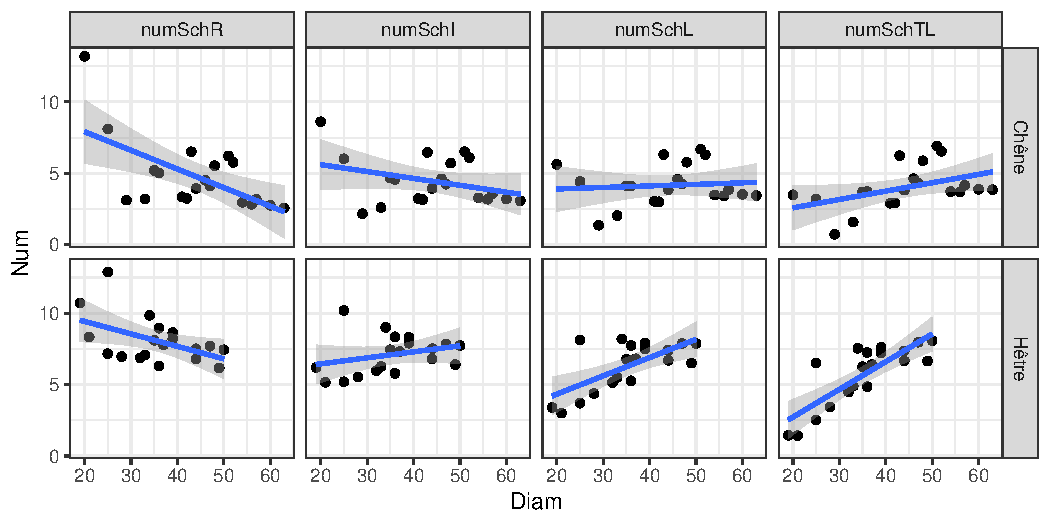
\includegraphics[width=\maxwidth]{Figures/FindSchGraph-1} 

}

\caption[Choix d'un tarif Schaeffer]{Choix d'un tarif Schaeffer.}\label{fig:FindSchGraph}
\end{figure}


\end{knitrout}

Le tableau n°\ref{FindSch} et la figure n°\ref{fig:FindSchGraph} montrent que pour cette application numérique, dans le cas du chêne il faudra utiliser un SchL n° 4.3 et un SchI n°7.3 pour le hêtre (numéros et types correspondants aux plus faibles coefficients de variation).


\subsubsection{Calcul d'erreur avec un tarif Schaeffer}\label{ParaErreurTarif}
La fonction \texttt{TarifErreurSch} calcule l'erreur liée à l'estimation du volume d'un lot par utilisation d'un tarif Schaeffer. A titre d'application numérique, le tableau \ref{DataErreurTarif} contient dans ses 2 premières colonnes l'échantillon d'arbres qui permet de trouver la moyenne des numéros et leur variance pour les 4 types de tarif Schaeffer, les 2 dernières colonnes correspondant au lot à cuber. Les données utilisées dans l'application numérique ci-après sont fournies avec le package \texttt{Forestree.}

% latex table generated in R 3.6.1 by xtable 1.8-4 package
% Wed May 20 14:10:38 2020
\begin{table}[ht]
\centering
\begingroup\small
\begin{tabular}{rrrr}
  \hline
Diam & Volume & Diam & Nombre \\ 
  \hline
47 & 1.344 & 20 & 1 \\ 
  43 & 1.299 & 25 & 3 \\ 
  51 & 1.914 & 30 & 5 \\ 
  52 & 1.940 & 35 & 6 \\ 
  35 & 0.707 & 40 & 2 \\ 
  29 & 0.362 & 45 & 2 \\ 
  46 & 1.319 & 50 & 1 \\ 
  54 & 1.687 &  &  \\ 
  42 & 0.950 &  &  \\ 
  25 & 0.345 &  &  \\ 
  63 & 2.322 &  &  \\ 
  60 & 2.112 &  &  \\ 
  48 & 1.579 &  &  \\ 
  57 & 1.950 &  &  \\ 
  56 & 1.813 &  &  \\ 
  41 & 0.905 &  &  \\ 
  36 & 0.750 &  &  \\ 
  44 & 1.130 &  &  \\ 
  33 & 0.515 &  &  \\ 
  20 & 0.227 &  &  \\ 
   \hline
\end{tabular}
\endgroup
\caption{Données utilisées pour le calcul d'erreur avec un tarif Schaeffer.} 
\label{DataErreurTarif}
\end{table}


\begin{knitrout}\small
\definecolor{shadecolor}{rgb}{0.969, 0.969, 0.969}\color{fgcolor}\begin{kframe}
\begin{alltt}
\hlkwd{data}\hlstd{(}\hlstr{"VolEchan"}\hlstd{,} \hlkwc{package} \hlstd{=} \hlstr{"DataForet"}\hlstd{)}
\hlkwd{data}\hlstd{(}\hlstr{"VolLot"}\hlstd{,} \hlkwc{package} \hlstd{=} \hlstr{"DataForet"}\hlstd{)}
\hlstd{tab} \hlkwb{<-} \hlkwd{TarifErreurSch}\hlstd{(VolEchan, VolLot)}
\end{alltt}
\end{kframe}
\end{knitrout}

% latex table generated in R 3.6.1 by xtable 1.8-4 package
% Wed May 20 14:10:38 2020
\begin{table}[ht]
\centering
\begingroup\small
\begin{tabular}{lrrr}
  \hline
Type & Num & Volume & Erreur \\ 
  \hline
SchI & 4.4 & 13.6 & 0.093 \\ 
  SchL & 4.2 & 13.8 & 0.081 \\ 
  SchR & 4.8 & 13.4 & 0.139 \\ 
  SchTL & 4.0 & 14.1 & 0.088 \\ 
   \hline
\end{tabular}
\endgroup
\caption{Volume estimé d'un lot d'arbres avec erreur associée.} 
\label{ErreurTarif}
\end{table}


A titre d'exemple la fonction \texttt{TarifErreurSch} renvoie le tableau n°\ref{ErreurTarif} qui fournit par type de tarif Schaeffer rapide, intermédiaire, lent ou très lent le numéro à utiliser, le volume du lot accompagné de son erreur d'estimation. Dans le cas de l'application numérique, c'est un tarif Schaeffer lent n° 4.2 qui conduira à l'erreur d'estimation la plus faible.

\subsection{Tarifs de cubage à deux entrées}

\subsubsection{Tarifs Chaudé}
Ils nécessitent la connaissance du diamètre à 1,3 m et de la hauteur découpe. Ils sont basés sur la formule suivante :
\begin{displaymath}
V(D,H,\delta) = \frac{\pi}{40000}*[D - \delta*(\frac{H}{2} - 1,3)]^2 * H
\end{displaymath}
où D est exprimé et cm, H en m et $ \delta $ en cm par mètre.
Il existe 20 tarifs Chaudé classiques numérotés de 1 à 20 caractérisés par une décroissance métrique sur le diamètre variable selon la classe de diamètre. Le choix d'un numéro revient à choisir la fonction de décroissance métrique (voir tableau n°\ref{decChaude}).


% latex table generated in R 3.6.1 by xtable 1.8-4 package
% Wed May 20 14:10:38 2020
\begin{table}[ht]
\centering
\begingroup\footnotesize
\begin{tabular}{rrrrrrrrrrrrrrrrrrrrr}
  \hline
Diam & 1 & 2 & 3 & 4 & 5 & 6 & 7 & 8 & 9 & 10 & 11 & 12 & 13 & 14 & 15 & 16 & 17 & 18 & 19 & 20 \\ 
  \hline
10 & 1.9 & 1.6 & 1.3 & 1.0 & 0.8 & 0.7 & 0.6 & 0.6 & 0.5 & 0.5 & 0.5 & 0.4 & 0.4 & 0.3 & 0.3 & 0.3 & 0.3 & 0.3 & 0.2 & 0.2 \\ 
  15 & 2.2 & 1.9 & 1.6 & 1.3 & 1.1 & 1.0 & 0.9 & 0.8 & 0.8 & 0.7 & 0.7 & 0.6 & 0.6 & 0.5 & 0.5 & 0.4 & 0.4 & 0.3 & 0.2 & 0.2 \\ 
  20 & 2.5 & 2.2 & 1.9 & 1.6 & 1.4 & 1.3 & 1.2 & 1.1 & 1.0 & 1.0 & 0.9 & 0.8 & 0.8 & 0.7 & 0.6 & 0.6 & 0.5 & 0.4 & 0.3 & 0.3 \\ 
  25 & 2.7 & 2.5 & 2.2 & 1.9 & 1.7 & 1.6 & 1.4 & 1.3 & 1.2 & 1.2 & 1.1 & 1.0 & 0.9 & 0.8 & 0.7 & 0.7 & 0.6 & 0.5 & 0.4 & 0.3 \\ 
  30 & 2.9 & 2.7 & 2.4 & 2.1 & 1.9 & 1.8 & 1.6 & 1.5 & 1.4 & 1.4 & 1.3 & 1.2 & 1.1 & 1.0 & 0.9 & 0.8 & 0.7 & 0.6 & 0.5 & 0.4 \\ 
  35 & 3.2 & 2.9 & 2.6 & 2.3 & 2.1 & 2.0 & 1.8 & 1.7 & 1.6 & 1.5 & 1.4 & 1.3 & 1.2 & 1.1 & 1.0 & 0.9 & 0.8 & 0.7 & 0.6 & 0.5 \\ 
  40 & 3.4 & 3.1 & 2.8 & 2.5 & 2.3 & 2.2 & 2.0 & 1.9 & 1.8 & 1.7 & 1.6 & 1.5 & 1.4 & 1.3 & 1.2 & 1.1 & 0.9 & 0.8 & 0.7 & 0.5 \\ 
  45 & 3.5 & 3.2 & 2.9 & 2.6 & 2.4 & 2.3 & 2.1 & 2.0 & 1.9 & 1.8 & 1.7 & 1.6 & 1.5 & 1.4 & 1.3 & 1.2 & 1.0 & 0.9 & 0.8 & 0.6 \\ 
  50 & 3.6 & 3.3 & 3.0 & 2.7 & 2.5 & 2.4 & 2.2 & 2.0 & 1.9 & 1.9 & 1.8 & 1.7 & 1.6 & 1.5 & 1.4 & 1.3 & 1.1 & 1.0 & 0.9 & 0.7 \\ 
  55 & 3.7 & 3.4 & 3.1 & 2.8 & 2.6 & 2.5 & 2.3 & 2.1 & 2.0 & 2.0 & 1.9 & 1.8 & 1.7 & 1.6 & 1.5 & 1.4 & 1.2 & 1.1 & 1.0 & 0.8 \\ 
  60 & 3.8 & 3.5 & 3.2 & 3.0 & 2.7 & 2.6 & 2.4 & 2.3 & 2.1 & 2.0 & 1.9 & 1.8 & 1.7 & 1.6 & 1.5 & 1.4 & 1.3 & 1.2 & 1.1 & 0.9 \\ 
  65 & 4.0 & 3.6 & 3.3 & 3.1 & 2.8 & 2.6 & 2.5 & 2.4 & 2.2 & 2.1 & 2.0 & 1.9 & 1.8 & 1.7 & 1.6 & 1.5 & 1.4 & 1.3 & 1.1 & 1.0 \\ 
  70 & 4.1 & 3.7 & 3.4 & 3.2 & 2.9 & 2.7 & 2.6 & 2.5 & 2.3 & 2.2 & 2.1 & 2.0 & 1.9 & 1.8 & 1.7 & 1.6 & 1.5 & 1.4 & 1.2 & 1.1 \\ 
  75 & 4.2 & 3.8 & 3.5 & 3.3 & 3.0 & 2.7 & 2.6 & 2.6 & 2.4 & 2.3 & 2.2 & 2.1 & 2.0 & 1.8 & 1.7 & 1.6 & 1.5 & 1.5 & 1.3 & 1.2 \\ 
  80 & 4.4 & 3.9 & 3.6 & 3.4 & 3.1 & 2.8 & 2.7 & 2.7 & 2.5 & 2.4 & 2.3 & 2.2 & 2.1 & 1.9 & 1.8 & 1.7 & 1.6 & 1.5 & 1.4 & 1.3 \\ 
  85 & 4.5 & 4.1 & 3.8 & 3.5 & 3.2 & 2.9 & 2.8 & 2.8 & 2.6 & 2.5 & 2.4 & 2.3 & 2.2 & 2.0 & 1.9 & 1.8 & 1.7 & 1.6 & 1.5 & 1.4 \\ 
  90 & 4.6 & 4.3 & 3.9 & 3.5 & 3.3 & 3.1 & 3.0 & 2.9 & 2.7 & 2.6 & 2.5 & 2.4 & 2.3 & 2.1 & 2.0 & 1.9 & 1.8 & 1.7 & 1.6 & 1.5 \\ 
  95 & 4.7 & 4.5 & 4.1 & 3.8 & 3.5 & 3.3 & 3.1 & 3.0 & 2.8 & 2.7 & 2.6 & 2.5 & 2.4 & 2.2 & 2.1 & 2.0 & 1.9 & 1.8 & 1.7 & 1.6 \\ 
  100 & 4.7 & 4.5 & 4.1 & 3.8 & 3.5 & 3.3 & 3.1 & 3.0 & 2.8 & 2.7 & 2.6 & 2.5 & 2.4 & 2.2 & 2.1 & 2.0 & 1.9 & 1.8 & 1.7 & 1.6 \\ 
   \hline
\end{tabular}
\endgroup
\caption{Décroissance métrique sur le diamètre (en cm/m) en fonction du diamètre pour les 20 tarifs classiques Chaudé.} 
\label{decChaude}
\end{table}


La fonction \texttt{TarifChaude} renvoie le volume calculé avec un tarif Chaudé à deux entrées. Le résultat est exprimé en m3. Le diamètre doit être exprimé en cm, la hauteur en m.
\begin{knitrout}\small
\definecolor{shadecolor}{rgb}{0.969, 0.969, 0.969}\color{fgcolor}\begin{kframe}
\begin{alltt}
\hlstd{Hauts} \hlkwb{<-} \hlkwd{c}\hlstd{(}\hlnum{13}\hlstd{,}\hlnum{14}\hlstd{,}\hlnum{14}\hlstd{)}
\hlstd{Diams} \hlkwb{=} \hlkwd{c}\hlstd{(}\hlnum{45}\hlstd{,}\hlnum{45}\hlstd{,}\hlnum{50}\hlstd{)}
\hlkwd{TarifChaude}\hlstd{(}\hlnum{13}\hlstd{, Diams, Hauts)} \hlcom{# cas d'un Chaudé n°13}
\end{alltt}
\begin{verbatim}
FALSE [1] 1.412925 1.460875 1.837552
\end{verbatim}
\end{kframe}
\end{knitrout}


\subsubsection{Tarifs Schaeffer à 2 entrées}
Ils sont moins connus que les tarifs de même nom à une entrée. Ils sont basés sur le coefficient de décroissance ($ k = D_m/D $). Ils se calculent à l'aide de la formule
\begin{displaymath}
V = \frac{\pi}{40000} * D^2_m * H = \frac{\pi}{40000} * k^2 * D^2 * H
\end{displaymath}

Pour les tarifs Schaeffer à 2 entrées, le coefficient de décroissance est fourni par la formule suivante.
\begin{displaymath}
k = \frac{a - b*H - k'C}{100}
\end{displaymath}
où, \\
- $ a $, $ b $ et $ k' $ sont des paramètres que l'utilisateur va devoir choisir parmi ceux proposés au tableau \ref{Schaeffer2Param} ;\\
-  $ H $ correspond à la hauteur découpe ;\\
- $ C $ à la circonférence exprimée en cm.\\

\begin{small}
\begin{table}[H]
\begin{tabular}{|c|r|r|r|l|l|}
\hline
\textbf{Num} & \multicolumn{1}{c|}{\textbf{a}} & \multicolumn{1}{c|}{\textbf{b}} & \multicolumn{1}{c|}{\textbf{k'}} & \multicolumn{1}{c|}{\textbf{Essences}} & \multicolumn{1}{c|}{\textbf{Commentaires}} \\ \hline
1 & 100 & 1,1 &   & Toutes & Très grosse découpe \\
2 & 97 & 1 &   & Chêne, hêtre & Massifs clairs, hauteurs corrigées \\
3 & 98 & 1,5 &   & Bouleau & Peuplement clair \\
4.1 & 100 & 1,8 &   & Peupliers & Bien élagués découpe de 60 à 120 cm au dessous de 12m \\
4.2 & 86,8 & 0,7 &   & Peupliers & Bien élagués découpe de 60 à 120 cm au dessus de 12m \\
5.1 & 96 & 1,8 &   & Peupliers & Mal élagués découpe de 60 à 120 cm au dessous de 12m \\
5.2 & 82,8 & 0,7 &   & Peupliers & Mal élagués découpe de 60 à 120 cm au dessus de 12m \\ \hline
6 & 93 & 0,5 & 0,03 & Sapins & Arbres élancés, découpe relativement forte \\
7 & 92 & 0,5 & 0,05 & Epicéas & Arbres à empattement marqué, découpe fine \\
8.1 & 93 & 1,6 &   & Ep, Mél, Pins & Plantation claire, inférieure à 10 m \\
8.2 & 82 & 0,5 &   & Ep, Mél, Pins & Plantation claire, supérieure à 10 m \\
9 & 80 & 0,25 &   & Pin sylvestre & Peuplements naturels Auvergne, découpe 10 cm \\
10 & 92 & 1,5 &   & Pin sylvestre & Plantation claire \\ \hline

\end{tabular}
\caption{Paramètres des tarifs Schaeffer à 2 entrées}
\label{Schaeffer2Param}
\end{table}
\end{small}

\begin{knitrout}\small
\definecolor{shadecolor}{rgb}{0.969, 0.969, 0.969}\color{fgcolor}\begin{kframe}
\begin{alltt}
\hlstd{Hauts} \hlkwb{<-} \hlkwd{c}\hlstd{(}\hlnum{13}\hlstd{,}\hlnum{14}\hlstd{,}\hlnum{14}\hlstd{)}
\hlstd{Diams} \hlkwb{=} \hlkwd{c}\hlstd{(}\hlnum{45}\hlstd{,}\hlnum{45}\hlstd{,}\hlnum{50}\hlstd{)}
\hlkwd{TarifSch2}\hlstd{(}\hlnum{2}\hlstd{, Diams, Hauts)} \hlcom{# cas d'un Schaeffer2 n°2}
\end{alltt}
\begin{verbatim}
FALSE [1] 1.458871 1.533907 1.893713
\end{verbatim}
\end{kframe}
\end{knitrout}

\subsubsection{Tarif EMERGE}
Le tarif EMERGE proposé par l'ONF est un tarif à deux entrées (hauteur totale et circonférence à 1,30 m) mais dont les coefficients dépendent de l'essence. Sa finalité est de calculer le volume total d'un arbre (volume total aérien, jusqu'à extrêmité des rameaux).
\begin{knitrout}\small
\definecolor{shadecolor}{rgb}{0.969, 0.969, 0.969}\color{fgcolor}\begin{kframe}
\begin{alltt}
\hlkwd{Tarif_EMERGE}\hlstd{(df, df}\hlopt{$}\hlstd{Haut, df}\hlopt{$}\hlstd{C130)}
\end{alltt}
\end{kframe}
\end{knitrout}

La fonction \textbf{\texttt{Vifn\_Vonf}} cartographie par sylvoécorégion le ratio entre le volume EMERGE et le volume géométrique bois fort tige de l'IFN.
\begin{knitrout}\small
\definecolor{shadecolor}{rgb}{0.969, 0.969, 0.969}\color{fgcolor}\begin{kframe}
\begin{alltt}
\hlstd{res} \hlkwb{<-} \hlkwd{Vifn_Vonf}\hlstd{(}\hlkwc{ess} \hlstd{=} \hlkwd{c}\hlstd{(}\hlstr{"02"}\hlstd{,}\hlstr{"03"}\hlstd{,}\hlstr{"05"}\hlstd{,}\hlstr{"06"}\hlstd{))}
\hlkwd{plot}\hlstd{(res}\hlopt{$}\hlstd{g)}
\end{alltt}
\end{kframe}
\end{knitrout}

\begin{figure}[H]
\begin{center}
 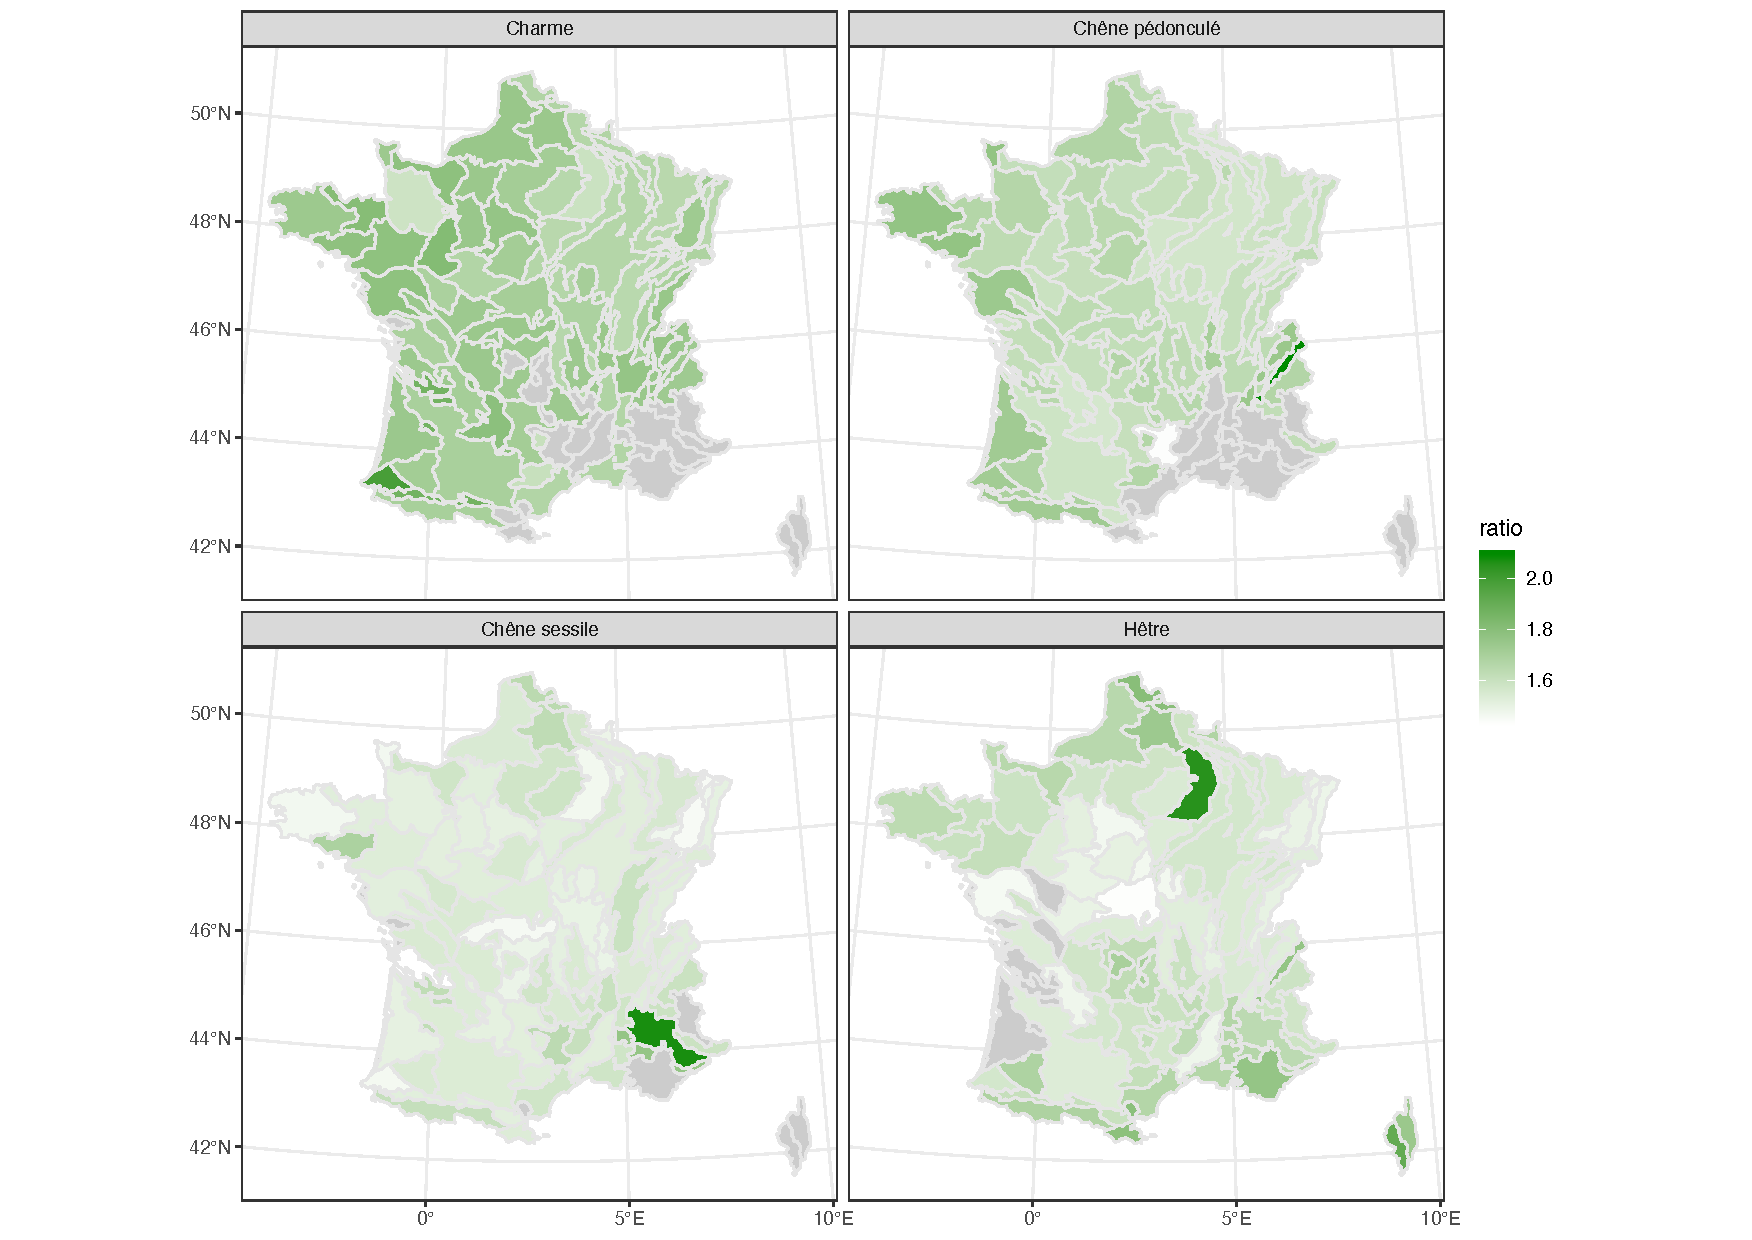
\includegraphics[width=17cm]{/Users/maxbruciamacchie/pCloud Sync/Packages/Forestree/Documentation/Figures/Emerge.pdf}
\caption{\emph{Ratio entre volume EMERGE et volume IFN.}}
\label{Emerge}
\end{center}
\end{figure}

La figure \ref{Emerge} permet de visualiser par sylvoécorégion le ratio entre le volume EMERGE et le volume géométrique bois fort tige de l'IFN.



\newpage
\subsection{Données IFN}

\subsubsection{Bases IFN}
Les bases de données arbres et placettes de l'IFN sont stockées dans le package DataForet. Elles sont accessibles avec l'instruction suivante. Des informations complémentaires sur les fonctions permettant d'exploiter les données de l'IFN se trouvent dans le package DataForet.

\begin{knitrout}\small
\definecolor{shadecolor}{rgb}{0.969, 0.969, 0.969}\color{fgcolor}\begin{kframe}
\begin{alltt}
\hlkwd{data}\hlstd{(}\hlstr{"IFNarbres"}\hlstd{,} \hlkwc{package} \hlstd{=} \hlstr{"DataForet"}\hlstd{)}
\hlkwd{data}\hlstd{(}\hlstr{"IFNplacettes"}\hlstd{,} \hlkwc{package} \hlstd{=} \hlstr{"DataForet"}\hlstd{)}
\end{alltt}
\end{kframe}
\end{knitrout}

\subsubsection{Accroissement sur le diamètre}
La fonction \textbf{\texttt{IFNacctD}} du package DataForet récupère dans la base de données de l'IFN les arbres vivants ne semblant pas avoir subi d'accident, ayant moins de 25 \% de branches mortes dans la partie supérieure du houppier qui ont directement accès à la lumière.

Le script suivant fournit les accroissements sur le diamètre pour l'ancienne forêt domaniale de Saint-Gobain (sans la partie Coussy-Basse).

\begin{knitrout}\small
\definecolor{shadecolor}{rgb}{0.969, 0.969, 0.969}\color{fgcolor}\begin{kframe}
\begin{alltt}
\hlcom{# ----------  données}
\hlkwd{data}\hlstd{(}\hlstr{"IFNarbres"}\hlstd{,} \hlkwc{package} \hlstd{=} \hlstr{"DataForet"}\hlstd{)}
\hlkwd{data}\hlstd{(}\hlstr{"IFNplacettes"}\hlstd{,} \hlkwc{package} \hlstd{=} \hlstr{"DataForet"}\hlstd{)}
\hlkwd{data}\hlstd{(}\hlstr{"CodesEssIFN"}\hlstd{,} \hlkwc{package} \hlstd{=} \hlstr{"DataForet"}\hlstd{)}
\hlkwd{data}\hlstd{(}\hlstr{"Ecorces"}\hlstd{,} \hlkwc{package} \hlstd{=} \hlstr{"DataForet"}\hlstd{)}
\hlkwd{data}\hlstd{(}\hlstr{"ser"}\hlstd{,} \hlkwc{package} \hlstd{=} \hlstr{"DataForet"}\hlstd{)}
\hlcom{# ---------- Choix}
\hlkwd{data}\hlstd{(}\hlstr{"FD"}\hlstd{,} \hlkwc{package} \hlstd{=} \hlstr{"DataForet"}\hlstd{)}
\hlstd{perim} \hlkwb{=} \hlstd{FD} \hlopt \hlkwd{filter}\hlstd{(IIDTN_FRT} \hlopt{==} \hlstr{"F10451Y"}\hlstd{)}
\hlcom{# ---------- Fonction}
\hlstd{acct} \hlkwb{<-} \hlkwd{IFNacctD}\hlstd{(perim)}
\hlcom{# ----------  Résultats}
\hlcom{# acct$tab}
\hlcom{# acct$Effectif}
\hlstd{acct}\hlopt{$}\hlstd{Graph}

\hlcom{# # ou bien choix du périmètre}
\hlcom{# acct <- IFNacctD()}
\end{alltt}
\end{kframe}\begin{figure}[h]

{\centering 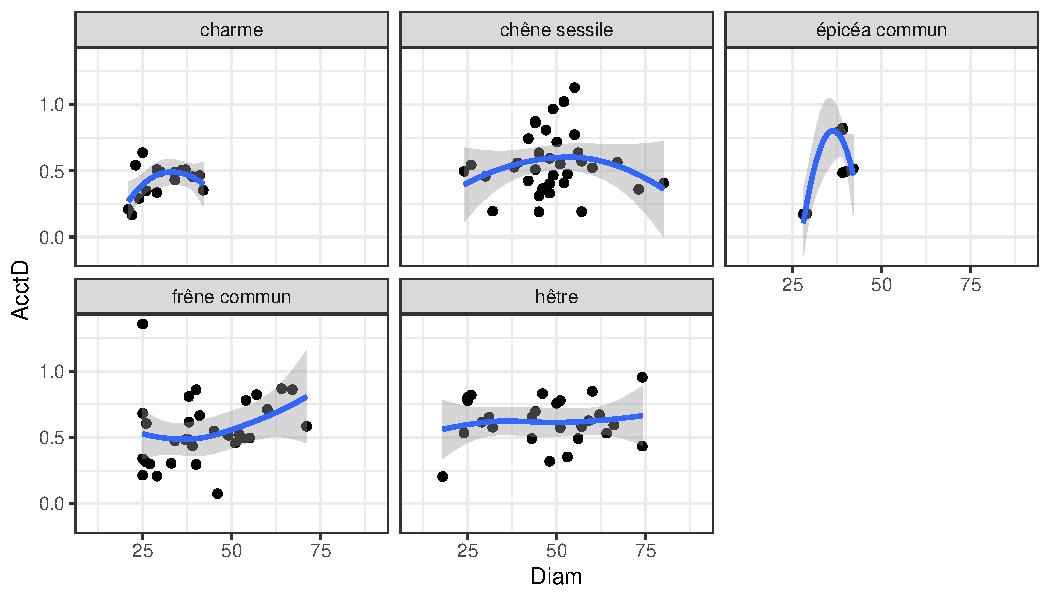
\includegraphics[width=\maxwidth]{Figures/IFNacctD-1} 

}

\caption[accroissements sur le diamètre pour l'ancienne forêt domaniale de Saint-Gobain]{accroissements sur le diamètre pour l'ancienne forêt domaniale de Saint-Gobain.}\label{fig:IFNacctD}
\end{figure}


\end{knitrout}


\subsubsection{Variables dendrométriques}
La fonction \texttt{IFNdendro} fournit une estimation de la surface terrière sur un périmètre choisi par l'opérateur : \\
- des principales essences ; \\
- de la structure en PER, PB, BM, GB ; \\
- de l'importance en BM + GB des deux essences contribuant le plus à la surface terrière totale. \\
Toutes ces informations sont accompagnées de leur coefficient de variation. Les calculs sont faits en supposant que toutes les placettes ont le même poids. \\
La fonction nécessite en entrée un shape correspondant au périmètre retenu : forêt, massif, sylvoécorégion, etc. Si le périmètre n'est pas indiqué, une boîte de dialogue permet de la choisir.

\begin{knitrout}\small
\definecolor{shadecolor}{rgb}{0.969, 0.969, 0.969}\color{fgcolor}\begin{kframe}
\begin{alltt}
\hlkwd{data}\hlstd{(perim)}
\hlkwd{load}\hlstd{(}\hlstr{"IFNdata.Rdata"}\hlstd{)}
\hlstd{res} \hlkwb{<-} \hlkwd{IFNdendro}\hlstd{(perim)}
\hlcom{# Résultats détaillés}
\hlstd{res}\hlopt{$}\hlstd{tab}        \hlcom{# Répartition de la surface terrière}
\hlstd{res}\hlopt{$}\hlstd{Nb}         \hlcom{# nombre de placettes IFN}
\hlstd{res}\hlopt{$}\hlstd{perimetre}  \hlcom{# périmètre retenu}
\hlstd{res}\hlopt{$}\hlstd{placettes}  \hlcom{# placettes IFN}
\end{alltt}
\end{kframe}
\end{knitrout}

\subsubsection{Cartographie des essences par sylvoécorégions}

\subsubsection{Cartographie des essences par sylvoécorégions}
La fonction fournit la répartition du volume d'une essence par classe de diamètre et par
région. Les deux découpages par régions sont ceux des GRECO ou des types de climats.

\begin{knitrout}\small
\definecolor{shadecolor}{rgb}{0.969, 0.969, 0.969}\color{fgcolor}\begin{kframe}
\begin{alltt}
\hlkwd{data}\hlstd{(IFNarbres)}
\hlkwd{data}\hlstd{(IFNplacettes)}
\hlkwd{data}\hlstd{(ser)}
\hlkwd{EvolEssence}\hlstd{(}\hlkwc{ess}\hlstd{=}\hlstr{"05"}\hlstd{,} \hlkwc{group}\hlstd{=}\hlstr{"climat"}\hlstd{)}
\end{alltt}
\end{kframe}
\end{knitrout}


\section{Milieux}

\subsection{Données climatiques}
\subsubsection{Diagramme ombrothermique}
La fonction \texttt{ClimatOmbro} permet l'édition d'un diagramme ombrothermique à partir d'informations mensuelles sur les températures et les précipitations. La figure \ref{fig:ClimatOmbro} présente un exemple.
\begin{knitrout}\small
\definecolor{shadecolor}{rgb}{0.969, 0.969, 0.969}\color{fgcolor}\begin{kframe}
\begin{alltt}
\hlstd{Precipitation} \hlkwb{=} \hlkwd{c}\hlstd{(}\hlnum{62}\hlstd{,}\hlnum{52}\hlstd{,}\hlnum{40}\hlstd{,}\hlnum{34}\hlstd{,}\hlnum{19}\hlstd{,}\hlnum{8}\hlstd{,}\hlnum{11}\hlstd{,}\hlnum{15}\hlstd{,}\hlnum{26}\hlstd{,}\hlnum{38}\hlstd{,}\hlnum{66}\hlstd{,}\hlnum{65}\hlstd{)}
\hlstd{Temperature} \hlkwb{=} \hlkwd{c}\hlstd{(}\hlnum{6.4}\hlstd{,}\hlnum{7.6}\hlstd{,}\hlnum{9.6}\hlstd{,}\hlnum{11.6}\hlstd{,}\hlnum{15.4}\hlstd{,}\hlnum{18.3}\hlstd{,}\hlnum{20.8}\hlstd{,}\hlnum{20.9}\hlstd{,}\hlnum{18.1}\hlstd{,}\hlnum{14.2}\hlstd{,}\hlnum{9.4}\hlstd{,}\hlnum{7.3}\hlstd{)}
\hlkwd{ClimatOmbro}\hlstd{(Temperature, Precipitation)}
\end{alltt}
\end{kframe}\begin{figure}[H]

{\centering 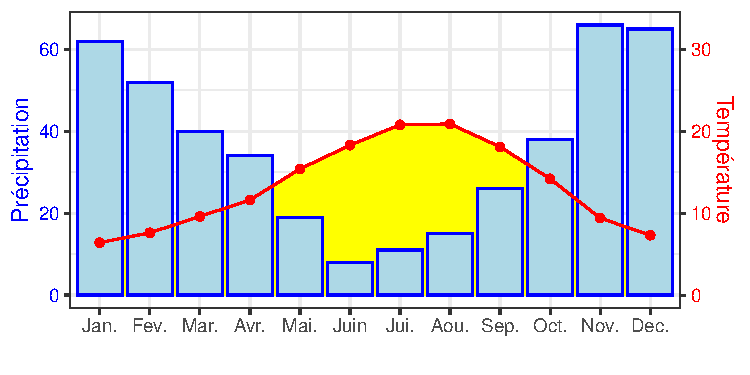
\includegraphics[width=\maxwidth]{Figures/ClimatOmbro-1} 

}

\caption[Exemple de diagramme ombrothermique]{Exemple de diagramme ombrothermique}\label{fig:ClimatOmbro}
\end{figure}


\end{knitrout}


% La fonction \texttt{ClimatOmbroMF} permet également l'édition d'un diagramme ombrothermique mais cette fois-ci à partir d'un d'un tableau contenant les informations classiques de météoFrance : Station, Année, Mois, RR (Précipitations), TN (témpérature minimale) et TX (température maximale). Si le tableau en entrée contient plusieurs stations, une boîte de dialogue permet de n'en sélectionner qu'une.

\begin{knitrout}\small
\definecolor{shadecolor}{rgb}{0.969, 0.969, 0.969}\color{fgcolor}\begin{kframe}
\begin{alltt}
\hlcom{##### Données}
\hlkwd{data}\hlstd{(}\hlstr{"DataMeteo"}\hlstd{)}
\hlcom{##### Visualisation}
\hlkwd{head}\hlstd{(DataMeteo)}
\hlcom{##### Utilisation fonction}
\hlkwd{ClimatOmbroMF}\hlstd{(DataMeteo)}
\end{alltt}
\end{kframe}
\end{knitrout}


\subsubsection{Rayonnement}
La quantité de rayonnement solaire conditionne le besoin en eau des plantes. La fonction \texttt{Rayonnement} nécessite en entrée le périmètre du territoire sous forme d'objet sf ainsi que son MNT. Elle renvoie un raster des écarts par rapport au rayonnement moyen.

\begin{knitrout}\small
\definecolor{shadecolor}{rgb}{0.969, 0.969, 0.969}\color{fgcolor}\begin{kframe}
\begin{alltt}
\hlkwd{library}\hlstd{(sf)}
\hlkwd{library}\hlstd{(tidyverse)}
\hlkwd{library}\hlstd{(raster)}
\hlkwd{library}\hlstd{(insol)}

\hlkwd{data}\hlstd{(razel)}
\hlstd{r} \hlkwb{<-} \hlkwd{SiteMnt}\hlstd{(razel)}
\hlstd{rad} \hlkwb{<-} \hlkwd{Rayonnement}\hlstd{(razel, r)}

\hlkwd{plot}\hlstd{(rad,} \hlkwc{axes}\hlstd{=F,} \hlkwc{box}\hlstd{=F)}
\hlkwd{plot}\hlstd{(}\hlkwd{st_geometry}\hlstd{(razel),} \hlkwc{add}\hlstd{=T)}
\hlcom{# writeRaster(rad, "Rad.tif", format="GTiff", overwrite=TRUE)}
\end{alltt}
\end{kframe}
\end{knitrout}

\subsubsection{EssenceClimat}
La fonction \textbf{\texttt{EssenceClimat}} permet de visualiser l'importance en volume d'une ou plusieurs essences selon le découpage de la France métropolitaine en 8 grands types de climat. Elle s'appuie sur la base IFN. Elle a comme argument la ou les essences retenues avec leur code IFN, ainsi le laps de temps sur lequel est calculée la moyenne des volumes. Par défaut les calculs portent sur les 7 dernières années.

\begin{knitrout}\small
\definecolor{shadecolor}{rgb}{0.969, 0.969, 0.969}\color{fgcolor}\begin{kframe}
\begin{alltt}
\hlkwd{library}\hlstd{(sf)}
\hlkwd{library}\hlstd{(tidyverse)}
\hlkwd{library}\hlstd{(DataForet)}
\hlkwd{library}\hlstd{(Forestree)}

\hlkwd{EssenceClimat}\hlstd{(}\hlkwd{c}\hlstd{(}\hlstr{"02"}\hlstd{,}\hlstr{"03"}\hlstd{,}\hlstr{"05"}\hlstd{,}\hlstr{"06"}\hlstd{))}
\hlkwd{EssenceClimat}\hlstd{(}\hlkwd{c}\hlstd{(}\hlstr{"09"}\hlstd{,}\hlstr{"61"}\hlstd{,}\hlstr{"62"}\hlstd{,}\hlstr{"52"}\hlstd{))}
\hlkwd{EssenceClimat}\hlstd{(}\hlstr{"09"}\hlstd{)}
\hlkwd{EssenceClimat}\hlstd{(}\hlkwd{c}\hlstd{(}\hlstr{"10"}\hlstd{,}\hlstr{"11"}\hlstd{))}
\end{alltt}
\end{kframe}
\end{knitrout}




% \subsubsection{Course du soleil}
% La fonction \texttt{CourseSoleil} renvoie la hauteur du soleil exprimée en degré au premier jour du printemps (20 mars) et de l'été (20 juin). Elle peut être utilisée pour calculer des masques solaires.
%
% <<CourseSoleil, fig.height=3, fig.pos='H', fig.cap="Hauteur du soleil en dégré à l'équinoxe de printemps et au solstice d'été.">>=
% library(tidyverse)
% library(suncalc)
%
% res <- CourseSoleil(Lat = 50.1, Lon = 1.83)
% res$graph
% @
%
%
% \subsection{Recherche statuts de protection}
% La fonction \texttt{NetProtectData} recherche sur internet les statuts de protection applicables sur un territoire donné. La fonction nécessite en entrée un fichier géoréférencé des limites du territoire au format sf ou shp. Si le fichier en entrée est au format shp, la fonction le transforme au format sf.
%
% Le tableau n°\ref{Liens} fournit la liste des liens internet recherchés
% <<Liens, echo=F, results='asis', fig.pos="H", comment=F>>=
% data(liens)
% print(xtable(liens, caption = "Statuts de protection : liens internet.",
%       digits=c(0,0,0),label = "Liens", caption.placement = "top"), include.rownames=F,
%       size="\\footnotesize")
% @
%
% La fonction \texttt{NetProtectData} va rechercher sur internet les fichiers géoréférencés des statuts de protection listés dans le tableau \ref{Liens}, fait une intersection avec les limites du territoire choisi et si le territoire est concerné par certains des statuts, crée un dossier dénommé StatutProtect contenant les shapes des intersections avec un buffer paramètrable (paramètre \texttt{width} de la fonction).
% <<eval=F, include=F>>=
% data(perim)
% NetProtectData(perim, width=500)
% @
%
% \begin{figure}[H]
% \begin{center}
%  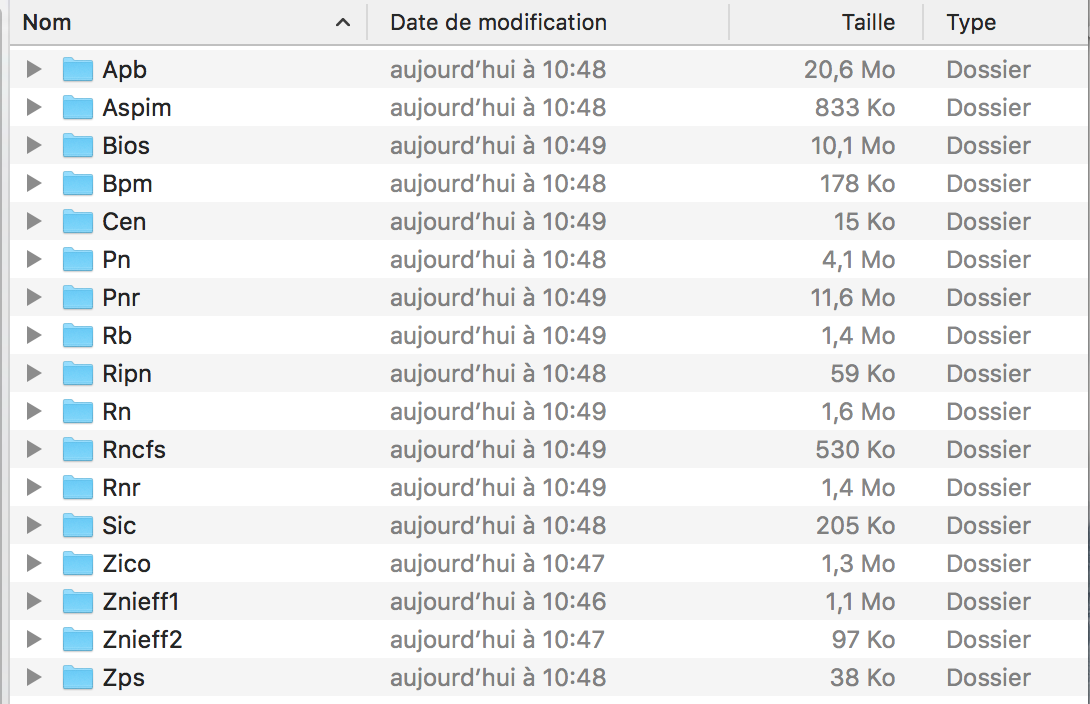
\includegraphics[width=10cm]{/Users/maxbruciamacchie/Dropbox/Packages/Forestree/Vignettes/Images/Protect.png}
% \caption{\emph{Résultat de la recherche des statuts de protection applicables sur un territoire donné.}}
% \label{Protec}
% \end{center}
% \end{figure}
%
%
% % \subsection{Géologie}
%
% \subsection{Topographie}
%
% \subsubsection{MNT}
% La topographie joue un rôle important dans la définition des stations et dans leur organisation spatiale. De nombreux indicateurs topographiques peuvent être calculés dès que l'on possède un modèle numérique de terrain. En France l'IGN met à disposition gratuitement un MNT à la résolution de 75 m. Il est possible, d'acheter auprès de l'IGN, des MNT au pas de 5 m. La NASA met à disposition des MNT (DEM en anglais) à la résolution de 30 m.\\
% Le package \texttt{elevatr} offre une alternative intéressante. Il permet de récupérer un MNT à partir d'une zone d'extension qui est calculée par le biais d'un polygone fourni en entrée. Avant janvier 2018 la recherche de MNT pouvait être faite sur 2 sources. Depuis une seule source est disponible, l'Amazon Web Services (aws).
%
% <<eval=F>>=
% library(elevatr)
% data(razel)
% # perim = st_read(dsn="/Users/bruciamacchiemax/Dropbox/Projets PSG/2018",
% #                 layer="Perim_Veyton")
% # r <- SiteMnt(perim)
% r <- SiteMnt(razel)
% par(mar=c(0,0,0,0))
% plot(r, axes=F, box=F)
% # plot(st_geometry(razel), add=T)
% plot(st_geometry(razel), add=T)
% @
%
% La fonction \texttt{SiteMnt} est basée sur la fonction \texttt{get\_elev\_raster} du package \texttt{elevatr} qui va rechercher sur le serveur de l'Amazon Web Services le raster correspondant à l'extension du spatialPolygon fourni en entrée. Le paramètre zoom doit être un entier. Il permet de choisir la résolution du raster en sortie. Sa valeur par défaut a été fixée à 14. Dans ce cas la résolution sera égale à environ 3,2 m. Si zoom est égal à 1 la résolution est de 7600 m, c'est pourquoi la fonction \texttt{SiteMnt} ramène automatiquement le zoom à 10 (résolution d'environ 51 m) si le zoom choisi par l'opérateur est inférieur à 10.\\
%
% La figure \ref{CompareMNT} permet de comparer le MNT de l'IGN vendu à une résolution de 5 m avec celui issu du serveur d'Amazon fourni avec une résolution annoncée légèrement supérieure à 3 m. La forêt retenue pour cette comparaison est située sur la commune d'Allevard en Isère, avec des altitudes comprises entre 500 et 2700 m. Cette figure montre que la résolution réelle d'Amazon est supérieure à 5m et que le mnt fourni par le serveur AWS a tendance à lisser le mnt réel. En utilisant les points géodésiques de l'IGN comme référence les écarts entre le mnt issu du serveur AWS et celui de l'IGN sont en moyenne comparable. Le principal intérêt du mnt issu du serveur AWS est que l'information est gratuite, disponible sur l'ensemble de la planète et de résolution largement suffisante pour de nombreux emplois en forêt.
%
% \begin{figure}[H]
% \begin{center}
%  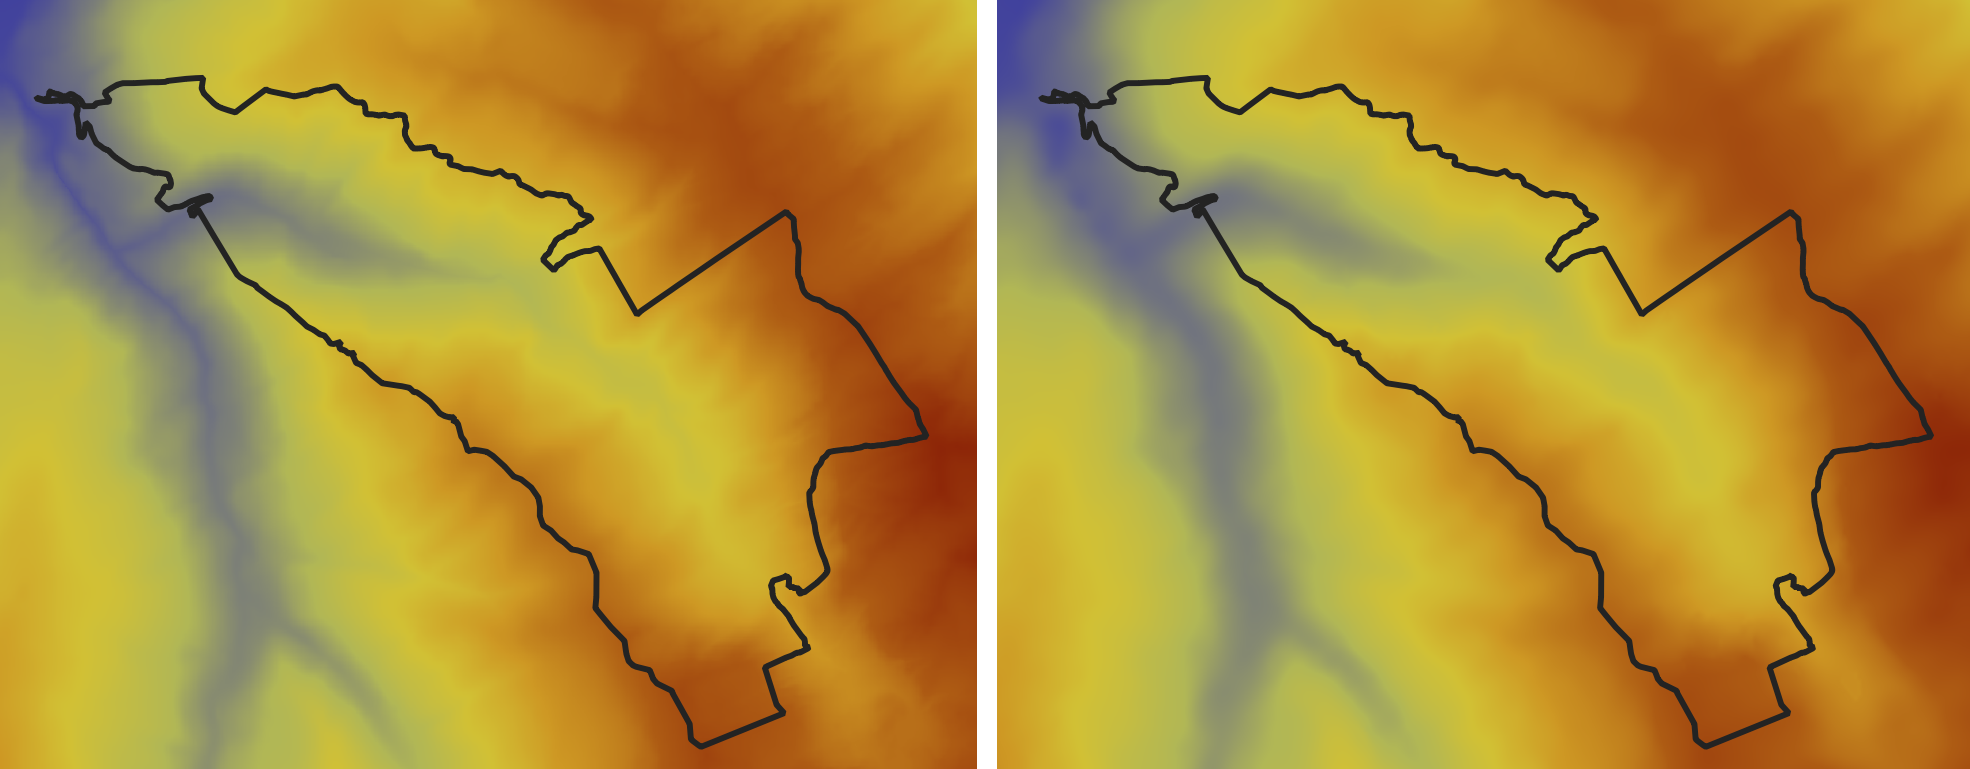
\includegraphics[width=17cm]{/Users/maxbruciamacchie/Dropbox/Packages/Forestree/Vignettes/Images/CompareMNT.png}
% \caption{\emph{Comparaison des résolutions entre le MNT de l'IGN (à droite) avec celui d'Amazon (à gauche)}}
% \label{CompareMNT}
% \end{center}
% \end{figure}
%
%
% \subsubsection{Indicateurs dérivés du MNT}
% La fonction \texttt{SiteTopo} permet de calculer des indicateurs topographiques sur un périmètre donné. Elle renvoie trois indicateurs topographiques : pente, classes de pente par exposition et direction de la ligne de plus grande pente.
% <<eval=F>>=
% library(raster)
% library(sf)
% library(tidyverse)
% library(scales)
%
% res <- SiteTopo(perim, mnt)
% res$Pente
% res$ExpoPente
% res$Ecoul
% @
%
% \begin{figure}[H]
% \begin{center}
%  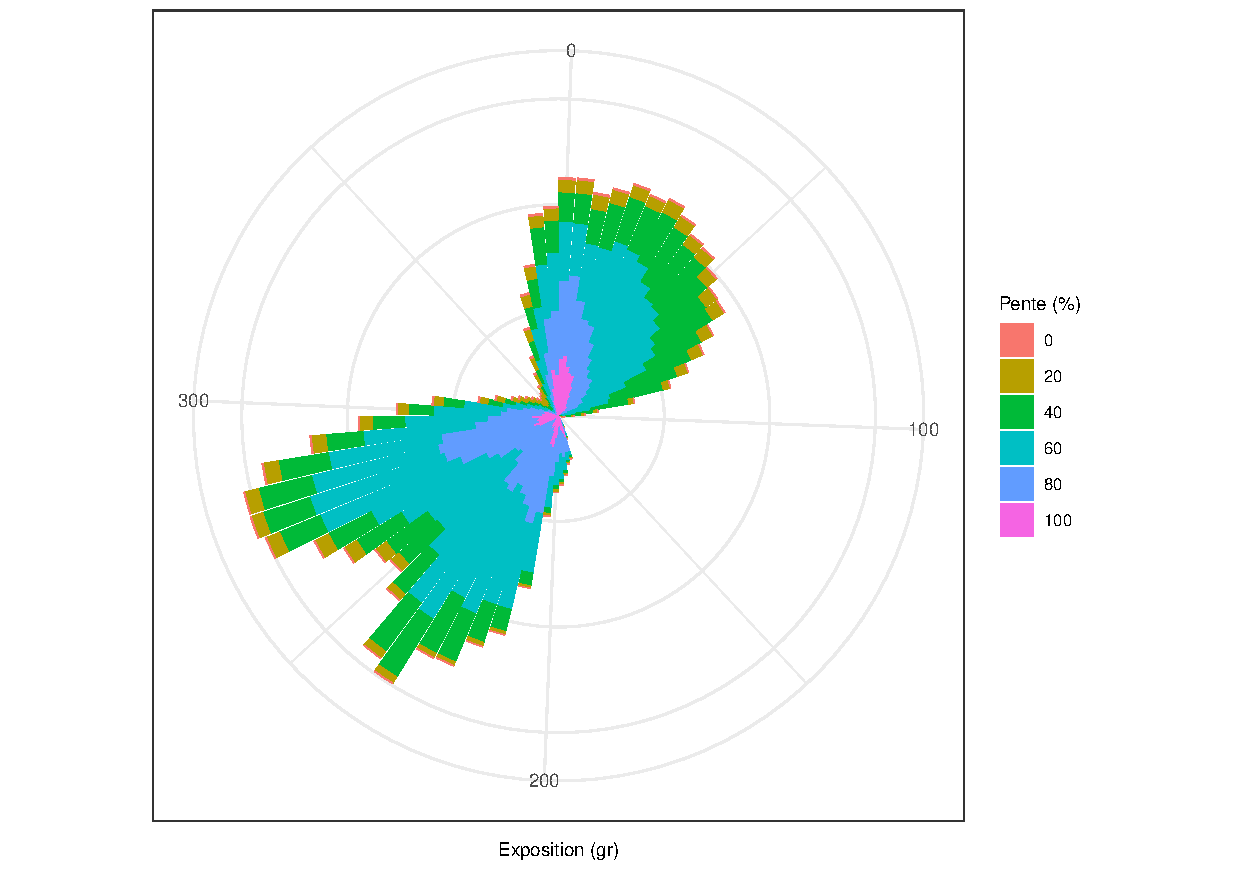
\includegraphics[width=15cm]{/Users/maxbruciamacchie/Dropbox/Packages/Forestree/Vignettes/Images/ClassePente.pdf}
% \caption{\emph{Exemple de répartition des pentes par exposition.}}
% \label{ClassePente}
% \end{center}
% \end{figure}
%
% \subsubsection{Fonction Countour2Line}
%
% <<Countour2Line, eval=F>>=
% library(sf, quietly =T, warn.conflicts =F)
% library(Forestree)
% data(razel)
% mnt = SiteMnt(razel)
% res <- Contour2Line(razel, mnt, valline="430")
% courbes <- res$courbes
% Ligne <- res$ligne
%
% plot(st_geometry(razel))
% plot(st_geometry(courbes), add=T, col='orange', lwd=0.5)
% plot(st_geometry(Ligne), add=T, col='red')
% @
%
% \begin{figure}[H]
% \begin{center}
%  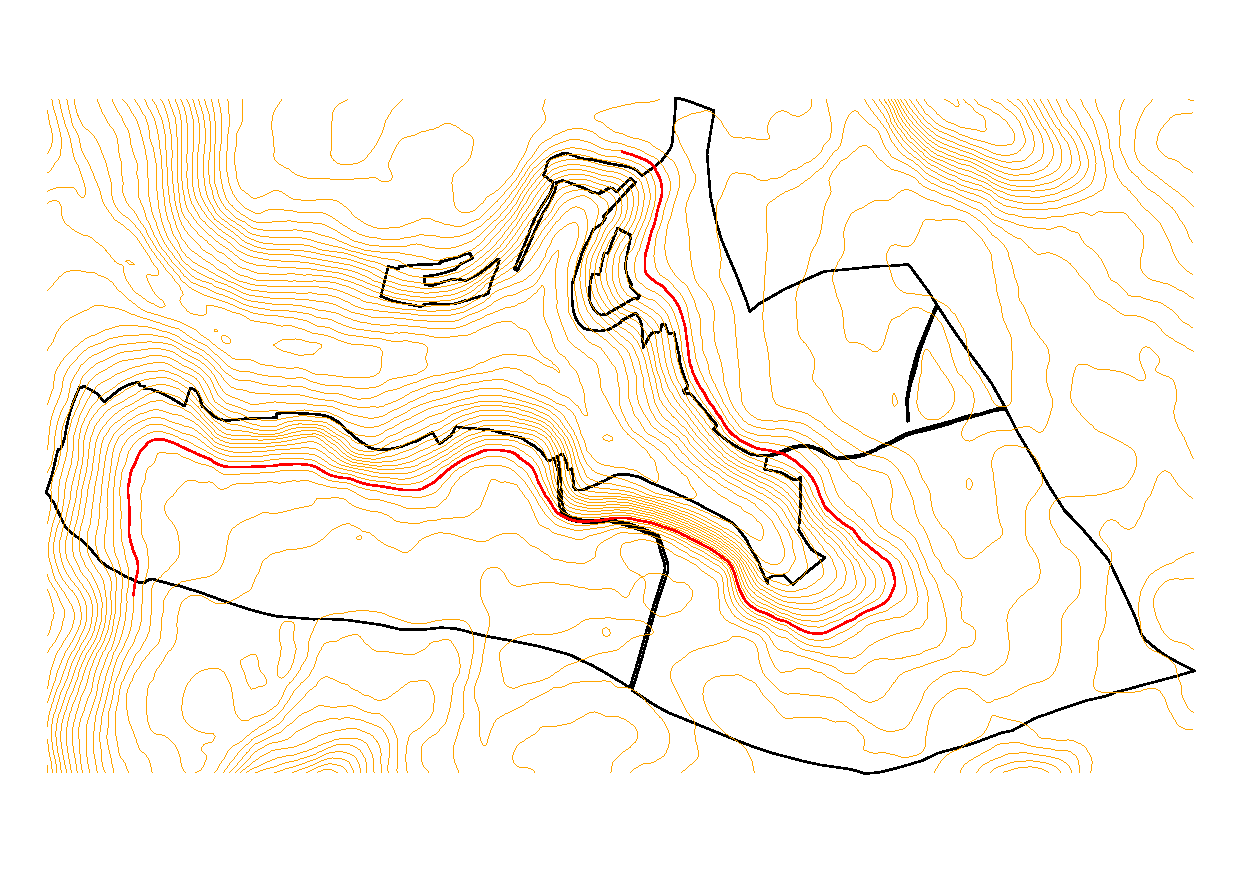
\includegraphics[width=15cm]{/Users/maxbruciamacchie/Dropbox/Packages/Forestree/Vignettes/Images/Courbes.pdf}
% \caption{\emph{Transformation d'un raster en courbes de niveau.}}
% \label{ClassePente}
% \end{center}
% \end{figure}
%
%
% \section{Gestion du foncier}
%
% \subsection{Conversion de matrices cadatrales en fichier Excel}
% La fonction \texttt{CadHtml2csv} permet la lecture de matrices cadastrales au format html contenues dans un dossier et renvoie un tableau contenant les informations suivantes : code et nom de la commune, nom et coordonnées du ou des propriétaires, identifiants des parcelles cadastrales, occupation du sol, revenu et surface cadastrals. Ces informations sont réparties dans les colonnes suivantes : COM\_CODE, COM\_NOM, PROP, ADRESSE, IDU, PREFIXE, SECTION, N\_PARCA, LIEUDIT, OCCUP\_SOL, REV\_CA, SURF\_CA.
%
% <<eval=F>>=
% tab <- CadHtml2csv(enrg=TRUE)
% @
%
% \subsection{Extraction des parcelles cadastrales}
% La fonction \texttt{CadPar} sélectionne dans un fichier .shp les parcelles cadastrales figurant dans des extraits de matrice cadastrale d'un ou de plusieurs propriétaires. Elle nécessite deux informations : \\
% - un tableau contenant la liste des parcelles cadastrales de la propriété. Il doit contenir une colonne nommée "idu" ou "IDU" ;\\
% - un fichier géoréférencé des parcelles cadastrales. Sa table attributaire doit contenir une colonne nommée "idu" ou "IDU".
% <<eval=F>>=
% data("MatriceCad")
% data("Parcellaire")
% cadastre <- CadPar(MatriceCad, Parcellaire)
% plot(st_geometry(cadastre), lwd=1.5, border='blue')
% @
%
%
% \subsection{Correspondance parcellaire forestier et cadastral}
%
% \subsubsection{La fonction CadCorFor}
% La fonction \texttt{CadCorFor} recherche la correspondance entre parcellaire forestier et cadastral. Elle fait en sorte que la somme des surfaces des parcelles forestières soit égale à la surface officielle cadastrale. Cette recherche est faite en évitant de trop aggréger les parcelles. Elle calcule un coefficient par parcelle permettant de passer de la surface SIG à la surface cadastrale.\\
%
% La fonction nécessite en entrée 2 fichiers géoréférencés au format sf : parcellaire cadastral et forestier. Si les fichiers en entrée sont au format shp, la fonction \texttt{st\_as\_sf} permet de les transformer au format sf (voir exemple ci-après).\\
%
% La table attributaire du parcellaire cadastral doit contenir au moins les champs suivants : Commune, Section, Num et Surface. Si la table attributaire du parcellaire forestier contient plusieurs colonnes, une boîte de dialogue permet de choisir le champ qui correspond au numéro de parcelle forestière.\\
%
% <<CadCorFor1, message=F>>=
% library(sf)
% library(Forestree)
% @
%
% \textbf{Données initiales}\\
% Dans la figure \ref{fig:CadCorFor2} les parcelles forestières sont en bleu, les parcelles cadastrales en rouge.\\
%
% <<CadCorFor2, warning=F, comment=F, error=F, fig.height=4, fig.cap="Parcellaire cadastral et forestier.">>=
% ##### Données
% data("parCadast")
% data("parFor")
% ##### Conversion du format shp au format sf
% parCadast <- st_as_sf(parCadast)
% parFor <- st_as_sf(parFor)
% ##### Visualisation
% par(mar=c(0,0,0,0))
% plot(st_geometry(parFor), lwd=2.5, border='blue')
% plot(st_geometry(parCadast), add=TRUE, border='red')
% @
%
% \textbf{Utilisation de la fonction}
% <<CadCorFor3, results='hide'>>=
% res <- CadCorFor(parCadast, parFor)
% @
%
% \textbf{Table de correspondance}\\
% Le tableau n°\ref{CadCorForTab} fournit la correspondance entre parcelles cadastrales et forestières.\\
% <<ResultTab, echo=F, results='asis', fig.pos="H", comment=F>>=
% print(xtable(res$Correspondance, caption = "Table de correspondance entre parcelles cadastrales et forestières.",
%       digits=c(rep(0,5)),label = "CadCorForTab", caption.placement = "top"), include.rownames=F,
%       size="\\footnotesize")
% @
%
% \textbf{Surface}\\
% Le tableau n°\ref{CadCorForSurf} fournit la surface cadastrale des parcelles forestières.
% <<ResultSurf, echo=F, results='asis', fig.pos="H", comment=F>>=
% print(xtable(res$Surfaces, caption = "Surface cadastrale des parcelles forestières.",
%       digits=c(0,0,4),label = "CadCorForSurf", caption.placement = "top"), include.rownames=F,
%       size="\\footnotesize", table.placement='H')
% @
%
% \subsubsection{La fonction CadPar}
% La fonction permet de produire un shapefile polygone contenant l'ensemble des parcelles cadastrales d'un ou plusieurs propriétaires. La fonction sélectionne dans un fichier .shp les parcelles cadastrales figurant dans des extraits de matrice cadastrale.
% <<CadParEx, fig.height=4, fig.pos="H", fig.cap="Exemple de visualisation des parcelles cadastrales d'une propriété.">>=
% data("MatriceCad")
% data("Parcellaire")
% shp <- CadPar(MatriceCad, Parcellaire)
% par(mar=c(0,0,0,0))
% plot(st_geometry(Parcellaire), border='blue', lwd=0.5)
% plot(st_geometry(shp), border='red', add=T)
% @
%
%
%
% \section{Données numériques}
% De plus en plus d'organismes mettent à disposition des données numériques. C'est le cas par exemple de l'IGN, du muséum d'histoire naturelles. Les données les plus anciennes sont en général gratuites, les données plus récentes et plus précises étant payantes. Des régions ou des départements ont créés des coopératives de données pour faciliter leur mise à disposition. C'est le cas de la région Grand-Est par le biais de son service CIGAL.
%
% \subsection{Découpes territoriales de la France}
%
% \subsubsection{Régions naturelles}
% La fonction \texttt{DecoupRN} met à disposition le découpage de la France en régions naturelles détaillées ou non par département, ainsi que le découpage en sylvoécorégions.
% <<CompareRN, fig.height=4, fig.pos='H', fig.cap="Comparaison entre anciennes régions naturelles (en bleu) et nouvelles sylvoécorégions (en rouge).">>=
% # anciennes régions naturelles
% # rn <- DecoupRN(formatSf = F, dept = F)
% # class(rn)
% # Compare anciennes régions naturelles et sylvoécorégions
% rn <- DecoupRN(formatSf = T, dept = F)
% data(ser)
% par(mar=c(0,0,0,0))
% plot(st_geometry(rn), border='blue', lwd=0.5)
% plot(st_geometry(ser), border='red', lwd=1.2, add=T)
% @
%
% \subsection{MNS ou MNH}
% \begin{minipage}{0.425\linewidth}
% Certaines collectivités territoriales mettent à disposition des gestionnaires de l'espace des données du type Modèle Numérique de Surface (MNS) issues d'un traitement LIDAR ou photogrammétrique. A titre d'exemple la figure \ref{Cigal} fournit les informations nécessaires pour se connecter au serveur FTP du CIGAL\footnote{Créé à l'origine par la région Alsace, les deux départements et les trois principales communautés urbaines, le CIGAL rassemble et met à disposition des données numériques pour l'ensemble de la nouvelle région Grand-Est}. \\
% Ayant récupéré le MNS auprès du CIGAL et à condition de posséder un Modèle Numérique de Terrain (MNT) suffisament précis (celui à une résolution de 5 convient parfaitement), il est possible de calculer par différence un Modèle Numérique de Hauteur (MNH = MNS - MNT). Ces modèles MNH peuvent être utilisé pour extrapoler des informations dendrométriques obtenues à partir d'inventaires en plein ou par placettes, aux espaces environnants (voir paragraphe \ref{ParaCarteGB}).
%
% \end{minipage}\hfill
% \begin{minipage}{0.55\linewidth}
% \begin{figure}[H]
% \begin{center}
%  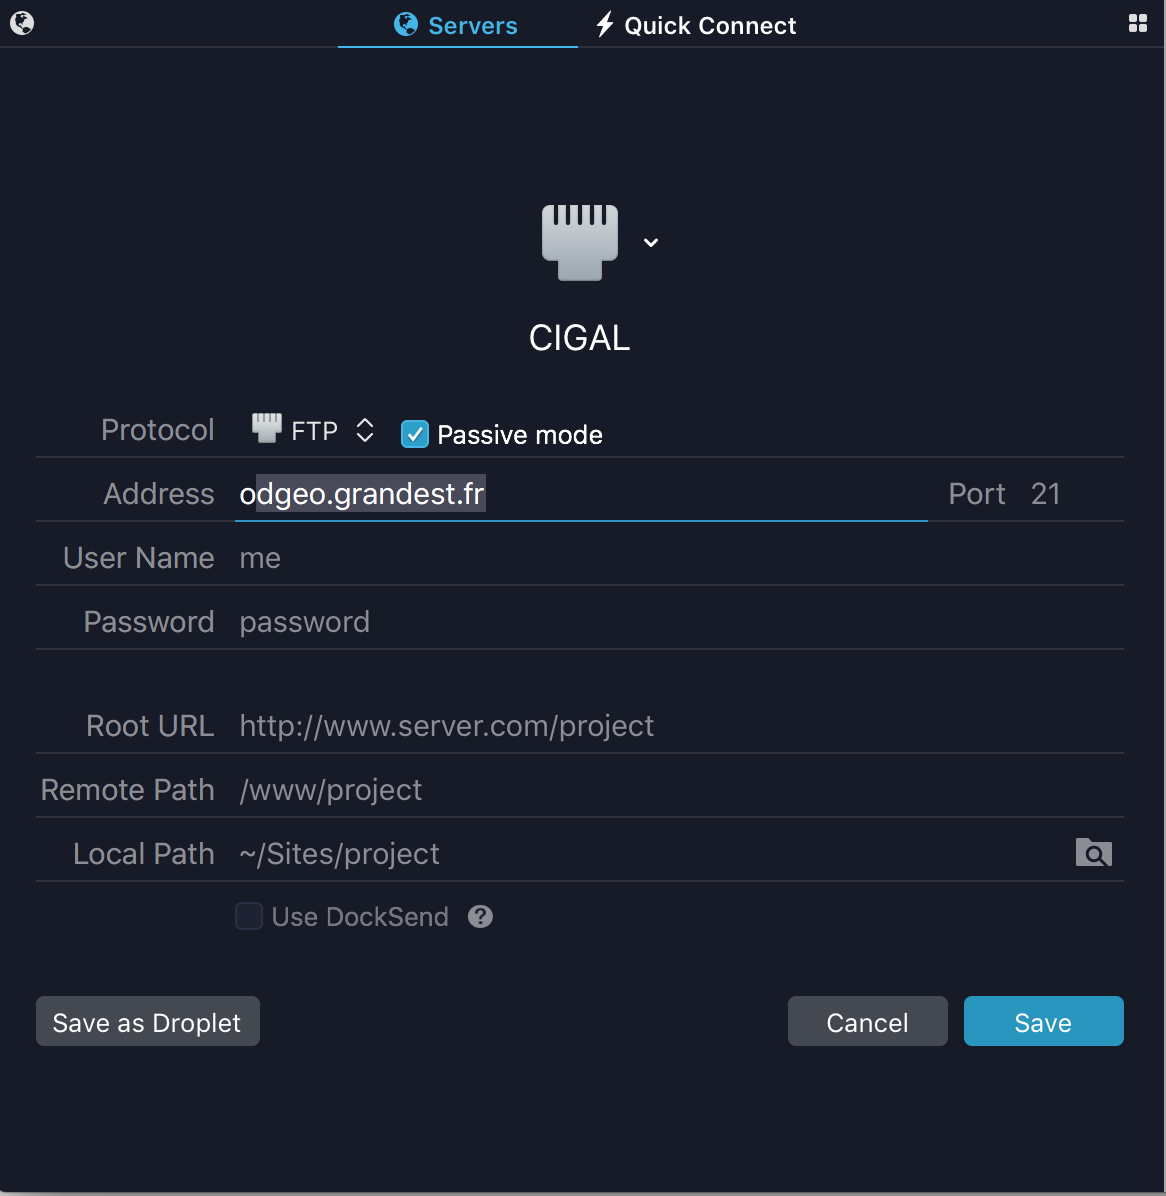
\includegraphics[width=8cm]{/Users/maxbruciamacchie/Dropbox/Packages/Forestree/Vignettes/Images/Cigal.png}
% \caption{\emph{Informations permettant de se connecter au serveur FTP du CIGAL.}}
% \label{Cigal}
% \end{center}
% \end{figure}
% \end{minipage}
%
% \subsubsection{Harmonisation}\label{ParaHarmo}
% Lorsque l'on souhaite utiliser ces données (MNS, MNT) qui se présentent génaralement sous forme de rasters, la première difficulté à surmonter est de les harmoniser car en général elles n'ont pas même résolution, point d'origine ou zone d'extension. C'est l'objectif de la fonction \texttt{HarmoniseRaster}.
% <<eval=F>>=
% data(mns)
% data(mnt)
% s <- HarmoniseRaster(mns, mnt)
% names(s) <- c("MNS", "MNT")
% # plot(s, axes=F, box=F)
% @
% La fonction \texttt{HarmoniseRaster} renvoie un objet de la classe "\texttt{RasterStack}".
%
% \subsubsection{Calcul du MNH}
%
% \begin{minipage}{0.55\linewidth}
% Les MNS et MNT harmonisés grâce à la fonction \texttt{HarmoniseRaster} (voir paragraphe \ref{ParaHarmo}) permettent par simple différence de calculer des Modèles Numériques de Hauteur (MNH). \\
%
% A titre d'exemple, la figure \ref{MNH17} permet de visualiser le MNH du dispositif n°17 (Belval) de l'AFI. L'échelle à droite est celle des hauteurs.
% <<eval=F>>=
% mns <- s$MNS
% mnt <- s$MNT
% mnh <- mns - mnt
% mnh[mnh<0] <- 0
%
% par(mar = rep(0.5, 4))
% plot(mnh, axes=F, box=F)
% plot(st_geometry(Parcelle), add=T)
% @
%
% \end{minipage}\hfill
% \begin{minipage}{0.425\linewidth}
% \begin{figure}[H]
% \begin{center}
%  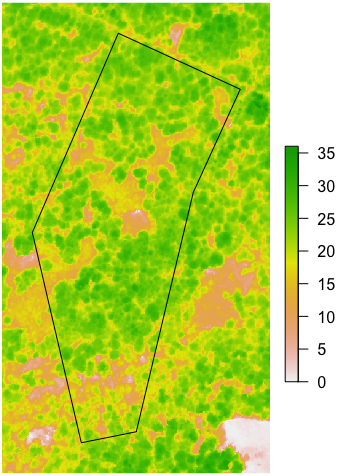
\includegraphics[width=6cm]{/Users/maxbruciamacchie/Dropbox/Packages/Forestree/Vignettes/Images/MNH17.png}
% \caption{\emph{Modèle Numérique de Hauteurs (MNH) - dispositif AFI n°17 (Belval).}}
% \label{MNH17}
% \end{center}
% \end{figure}
% \end{minipage}
%
% \subsubsection{Détection des arbres}\label{Detect}
% \begin{minipage}{0.525\linewidth}
% Le package \texttt{ForestTools} contient des fonctions permettant d'automatiser la détection à partir de MNH d'arbres (\texttt{TreeTopFinder}) ou de houppiers (\texttt{SegmentCrowns}). La recherche d'arbres est basée sur la détection des apex (points hauts). \\
% <<eval=F>>=
% lin <- function(x){-3 + 0.2*x}
% ttops <- vwf(CHM = mnh,
%              winFun = lin,
%              minHeight = 20,
%              maxWinDiameter = 30)
% crownsPoly <- mcws(treetops = ttops,
%                    CHM = mnh,
%                    format = "polygons",
%                    minHeight = 20,
%                    verbose = F)
% par(mar = rep(0.5, 4))
% plot(mnh, axes=F, box=F)
% plot(st_geometry(Parcelle), add=T)
% plot(crownsPoly, border = "blue", lwd = 0.2,
%      add = TRUE)
% plot(ttops, add=T, pch=19, col='blue',cex=0.2)
% @
% \end{minipage}\hfill
% \begin{minipage}{0.45\linewidth}
% \begin{figure}[H]
% \begin{center}
%  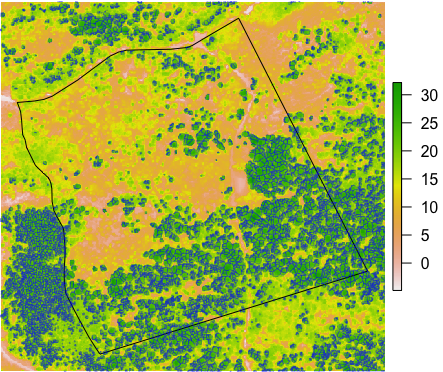
\includegraphics[width=6cm]{/Users/maxbruciamacchie/Dropbox/Packages/Forestree/Vignettes/Images/Houppier.png}
% \caption{\emph{Détection automatique des houppiers des arbres pour le dispositif AFI n°17 (Belval).}}
% \label{Houppier17}
% \end{center}
% \end{figure}
% \end{minipage}
%
% A titre d'exemple, la figure \ref{Houppier17} illustre le résultat de la détection automatique des houppiers dans le cas du dispositif n°17 (Belval) de l'AFI. Dans le script ci-dessus la fonction \texttt{lin} définit le rayon minimum de recherche du prochain apex. Elle a été établie à partir des mesures de houppiers effectuées à l'AFI. Ne sont recherchés que les arbres dont la hauteur est supérieure au paramètre à 20 mètres (paramère \texttt{minHeight}), valeur seuil également définie à partir des mesures de l'AFI.
%
%
% \subsubsection{Calibration}
% La détection des arbres à partir de MNH présentée au paragraphe \ref{Detect} n'est souvent qu'une première étape en vue d'estimer la ressource en volume. Elle nécessite d'établir des relations d'estimation du volume d'un arbre à partir de la surface de son houppier et de sa hauteur. \\
%
% Une autre approche consiste à établir une relation entre la distribution locale des hauteurs et une variable dendrométrique. A titre d'exemple la variable à prédire sera la surface terrière des gros bois. Cette seconde approche ne nécessite pas l'étape de la détection des arbres et de leur houppier.\\
%
% \begin{minipage}{0.55\linewidth}
% Un réseau de placettes permanentes va servir à calibrer une relation entre la distribution des hauteurs à partir du MNH, sur les cercles de 10m et de 30m, et la surface terrière des gros bois mesurée sur les placettes permanentes.
% <<eval=F>>=
% data(mnh)
% data(Parcelle)
% data(Placettes)
% plot(mnh, axes=F, box=F)
% plot(st_geometry(Parcelle), add=T)
% plot(st_geometry(Placettes), add=T)
% @
% \end{minipage}\hfill
% \begin{minipage}{0.45\linewidth}
% \begin{figure}[H]
% \begin{center}
%  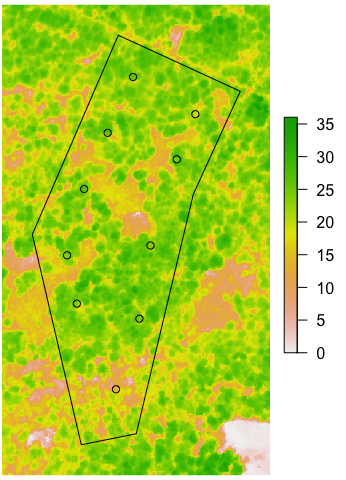
\includegraphics[width=6cm]{/Users/maxbruciamacchie/Dropbox/Packages/Forestree/Vignettes/Images/PlanPlacettes.png}
% \caption{\emph{Localisation des placettes permanentes - dispositif AFI n°17 (Belval).}}
% \label{Houppier17bis}
% \end{center}
% \end{figure}
% \end{minipage}
%
%
%
%
%
% \subsubsection{Carte de la surface terrière de gros bois}\label{ParaCarteGB}
% \begin{figure}[H]
% \begin{center}
%  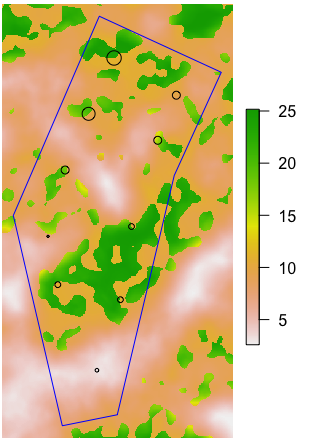
\includegraphics[width=6cm]{/Users/maxbruciamacchie/Dropbox/Packages/Forestree/Vignettes/Images/GB.png}
% \caption{\emph{Carte de la surface terrière de gros bois - dispositif AFI n°17 (Belval).}}
% \label{GB17}
% \end{center}
% \end{figure}
%
%
% \section{Estimation forestière}
%
% \subsection{Indicateurs économiques}
%
% \subsubsection{Pouvoir d'achat}
%
% <<eval=F>>=
% library(Forestree)
% library(dplyr)
% Coeft <- PouvoirAchat(2018)
% # ---- Exemple
% Flux <- data.frame(Année = c(1995, 1999, 2003, 1995:2003),
%                       Nature = c("Investissement", "Chasse", "Bois", rep("Frais fixe", 9)),
%                       Montant = c(-15000, 6000, 7000, rep(-50, 9))) %>%
%   arrange(Année) %>%
%   left_join(Coeft, by = "Année") %>%
%   mutate(MontantEuroCons = Montant * Coefft)
% sum(Flux$MontantEuroCons)
% @
%
% \subsubsection{Prix de vente des forêts}
% Par décret n° 2018-1350 du 28 décembre 2018, le gouvernement français s'est engagé à mettre en open data les informations portant sur les valeurs foncières déclarées à l'occasion des mutations immobilières. La base de donnée DVF (demandes de valeurs foncières), publiée et produite par la direction générale des finances publiques est donc accessible sur le serveur \emph{data.gouv.fr}. En pratique les informations se présentent sous la forme d'un fichier par année. Une ligne de chaque fichier représente un bien (appartement, parcelle cadastrale, etc.) présent dans une transaction. Les fichiers font l’objet d’une mise à jour semestrielle, en avril et en octobre. Les deux départements d'Alsace ainsi que la Moselle ne figurent pas dans la base de données. \\
%
% La base de donnée DVF n'est pas facilement manipulable car très volumineuse et mal organisée. La fonction \texttt{ValeurVenale} en facilite l'exploration. Elle ne retient que les ventes qui ne concernent que des parcelles cadastrales boisées (pas de bâti, de champ, etc.). Les DOM-TOM ont été volontairement retirés de l'analyse. \\
%
% Le script ci-après fournit un exemple d'utilisation. La figure \ref{fig:Valeurs} présente une des sorties possibles. Elle doit être interprétée en sachant que la nature de bois indiqué par le cadastre peut être assez éloignée de la réalité. Malgré cette réserve La figure \ref{fig:Valeurs}
% <<eval=F>>=
% library(tidyverse)
%
% Evol <- data.frame()
% Detail <- data.frame()
% for (i in c(2018:2016)) {
%   res  <- ValeurVenale(i)
%   Evol <- rbind(Evol, as.data.frame(res$tab))
%   Detail <- rbind(Detail, as.data.frame(res$Detail))
% }
%
% textes <- Evol %>% filter(Année == 2018)
% ggplot(Evol, aes(x=Nature, y=Prix, color=factor(Année))) +
%   geom_point() + geom_text(data=textes, aes(label=round(Prix,0)), size=4, hjust=1.2) +
%   theme_bw() + labs(color="")
%
% ggplot(Detail, aes(x=Nature, y=Prix, fill=factor(Année), color=factor(Année))) +
% geom_point(position = position_jitterdodge()) +
%   geom_boxplot(alpha=0.4) +
%   geom_text(data=textes, aes(label=round(Prix,0)), size=3, hjust=-1.5) +
%   theme_bw() + labs(fill="", color="", y="Prix (euro/ha)")
% @
%
% \begin{figure}[H]
% \begin{center}
%  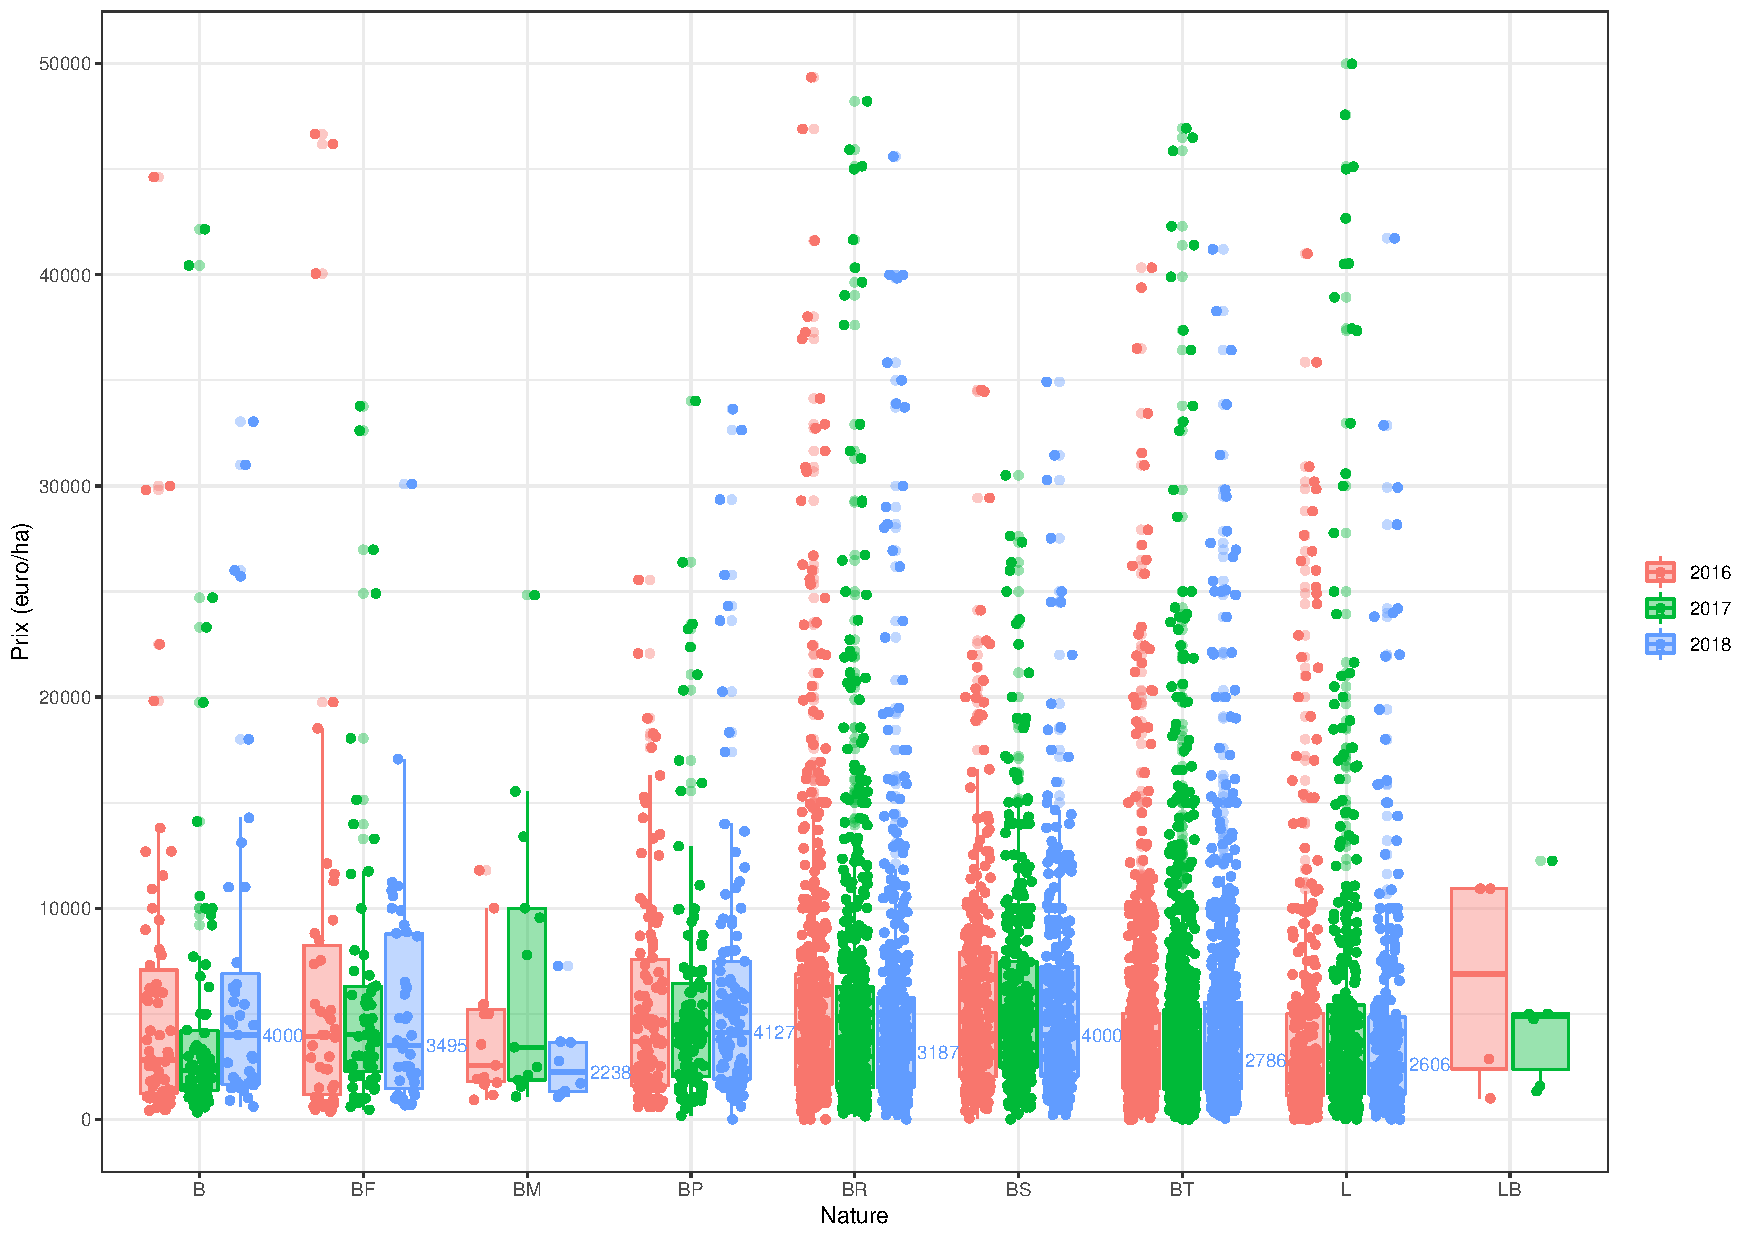
\includegraphics[width=17cm]{/Users/maxbruciamacchie/Dropbox/Packages/Forestree/Vignettes/Images/Valeurs.pdf}
% \caption{\emph{Valeurs des forêts selon leur nature (codification cadastrale)}}
% \label{Valeurs}
% \end{center}
% \end{figure}
%
%
% \subsubsection{taux interne de rentabilité}
% <<eval=F>>=
% df <- data.frame(Année = c(2, 4, 6, 30),
%                  Montant = c(-0.6, -0.9, -1.5, 9))
% EcoTIR(df$Année, df$Montant)
% @
%
% \subsection{Rentabilité de projets}
%
% \section{Gestion des risques}

\end{document}
